% Created 2021-06-24 Thu 14:39
% Intended LaTeX compiler: pdflatex
\documentclass[11pt]{article}
\usepackage[utf8]{inputenc}
\usepackage[T1]{fontenc}
\usepackage{graphicx}
\usepackage{grffile}
\usepackage{longtable}
\usepackage{wrapfig}
\usepackage{rotating}
\usepackage[normalem]{ulem}
\usepackage{amsmath}
\usepackage{textcomp}
\usepackage{amssymb}
\usepackage{capt-of}
\usepackage{hyperref}
\author{Filipa  Calado}
\date{\today}
\title{}
\hypersetup{
 pdfauthor={Filipa  Calado},
 pdftitle={},
 pdfkeywords={},
 pdfsubject={},
 pdfcreator={Emacs 26.2 (Org mode 9.1.9)}, 
 pdflang={English}}
\begin{document}

\tableofcontents

\section{one}
\label{sec:org85061e9}

\subsection{chapter summary}
\label{sec:orgaf9352c}
The burden of this chapter is to describe how to do text analysis in a
way that attends to queer concepts of gender performativity, and how
that method might leverage computational processes to analyze literary
material that express complex gender ontologies. I begin the chapter
by debunking what I call "the fantasy of falsifiable criticism," which
includes distant reading practicies by Franco Moretti and Ted
Underwood, constrasting their work with that of Richard Jean So and
Laura Mandell, whose methods emphasize deconstructing social
categories. While this deconstruction is important, I'm interested in
analysis of text that disrupts what we know about these literary
materials by creating new forms for understanding phenomena such as
gender ontolgies. For the middle portion of the chapter, I embark on
three "close-readings" of computer programming, gender theory, and my
source text, \emph{Orlando: A Biography} by Virginia Woolf. First, I delve
into python programming, focusing on the structure of the \texttt{for loop}
and processes for cleaning and regularizing text, with the goal of
bringing out the recursive quality of running python code. Then, I dip
into Judith Butler's concept of gender performativity, which lends an
understanding to the ways that critical processes can subvert dominant
structures through iteration, or what she calls "performative
citation." To wrap up this section, I do a close-reading of Woolf's
\emph{Orlando} that examines the ways that gender is closely coordinated
with the significatory power of language throughout the novel. In the
final section of the chapter, I apply Butler's notion of displacement
through repetition in gender performativity back to text analysis to
illustrate how the iterative process of analyzing text can surface new
textual structures that re-signify certain elements of that text. The
chapter ends with my text analysis of Virginia Woolf's \emph{Orlando} to
demonstrate how "man" and "woman" in that text is re-signified from
its initial binary structure into a plural understanding 


\subsection{The fantasy of the falsifiable}
\label{sec:orgb446226}

This chapter examines how quantitative text analysis, which is a way
of analyzing textual data by counting its features or elements, such
as calculating word frequency or generating associative word pairs,
works with data about gender ontology. This examination probes the
central tension between "Queer Form," or figurative and narrative
forms by which gender is expressed [further elaborated in the
introductory chapter], and digital formats, where the logics
computation abstracts and transforms text into data. The process of
preparing a text for text analyis always requires a reduction of data
in which some semantic value has escaped. Common tasks like cleaning
and normalizing, where text is transformed into a format to make it
computable, constrain textual meaning by passing text through an
automated seive, filtering out its specificities. For example, in
order to be counted in a word frequency, text has to be rid of
elements like punctuation, articles, prepositions, and word
endings. Rather than attempt to recover semantic escape, I am
interested in exploring how possible approaches for quantification
might engage with gender as a complex phenomenon.

Distant Reading is a way of computing textual data by cleaning,
sorting, and counting textual elements, and can involve more advanced
processes like statistical modelling and machine learning. It borrows
from quantitative methods in the social sciences, applying them to
textual data, for example in word association, topic modeling and
sentiment analysis. Though they differ in their specifics, these
methods share a faith in using the speed of computation, which can
process very precise elements like word frequency or syntactic
patterns, to make calculations about how to categorize or organize
textual data. Moreover, they are part of a scientific method meant to
guide researchers in conducting experiments that prove or falsify
their hypotheses. The scientific method is a cyclical process, wherein
researchers make observations on a certain topic, formulate a
hypothesis, test the hypothesis with experiments, analyze and report
the results, bringing them toward new observations, hypotheses,
experiments, and conclusions.

Franco Moretti, who is largely responsible for popularizing the
practice of Distant Reading in English Studies contexts, greatly
influenced the ways that English scholars approach quantiative
methodologies. Because computers can process hundreds of texts at a
time, "reading" at much faster rates than humans, they offer critics
an opportunity for getting around the problem of literary scale, and
particularly attract critics like Moretti who pose ambitious questions
about literary history. Moretti's scholarship explores how social and
economic forces impact literary form in the development of the modern
novel. His subject is the vast swatch of modern literary history,
thousands of texts that would otherwise be too large and unweildy to
work with. He declares that "distance \ldots{} is a condition of knowledge"
(\emph{Distant Reading} 48). Other scholars follow a similar path. More
recently, Ted Underwood, in the field of Computational Literary
Studies (CLS), harnesses the power of quantification and machine
learning to glimpse what he calls the "distant horizon" of literary
trends across centuries\footnote{Underwood, Ted. \emph{Distant Horizons}, 2019.; Underwood,
Ted. “Machine Learning and Human Perspective.” PMLA, Vol. 35 No. 1,
January 2020, pp. 92-109.}. Some recent developments in distant
reading combine with close reading methods, as critics will use the
results of quantitative analysis to identify key moments from the text
that merit closer attention.\footnote{Andrew Piper's methodology, which he calls "bifocal" reading,
demonstrates how distant and close reading are used together, with
distant reading providing the context or framework that guides close
reading"“We are no longer using our own judgments as benchmarks\ldots{} but
explicitly constructing the context through which something is seen as
significant (and the means through which significance is
assessed)\ldots{}. It interweaves subjectivity with objects” (Piper,
Andrew. Enumerations: Data and Literary Study, 2018, 17).}

I begin with Moretti, because it is important to examine where the
impulse for reading distantly emerges in his work. In Moretti's early
essay, "The Soul and the Harpy" (1983),\footnote{Moretti, Franco. "The Soul and the Harpy." \emph{Signs Taken For
Wonders: On the Sociology of Literary Forms}, trad. David Forgacs, New
York, Verso, 1983, pp. 1-41} he divulges a key motive
in developing his methodological approach, which will eventually
flourish into "distant reading." Underlying Moretti’s methodology is a
deep concern with finding a way to ascertain the effect of historical
forces on literary form. But the current practices of literary
criticism present methodological obstacle. In this early essay,
Moretti characterizes literary criticism as "a sort of cultivated
accompaniment to reading – to the reading we are doing here and now,"
("The Soul and the Harpy" 21). By this, he means that the analytical
practices of contemporary literary critics, which "revolve around
concepts such as ‘ambiguity’ and the like," will, according to
Moretti, "always be pushed into multiplying, rather than reducing, the
obstacles every social science encounters when it tries to give itself
a testable foundation" (22). To illustrate the practices of current
literary criticism, Moretti distinguishes between the historian and
the student of literature:
\begin{quote}
The [student] – unless desirous of turning into that legendary figure
whose only pleasure lay in contemplating his own reflection – must
concentrate on the dissimilarities and ruptures: on what has been lost
and become irretrievably unfamiliar, and which we can 're-familiarize'
only by doing such violence to it that we distort the objective,
material consistency of every work which it is the task of scientific
knowledge to reconstruct and 'salvage'. 14
\end{quote}
According to Moretti, the great danger in literary criticism is the
encouragement of narcissistic tendencies in researchers, whose attempt
to "re-familiarize" the object of study does it "violence". Moretti's
proposed method therefore would take a scientific approach that
maintains the "objective, material consistency" of the work. Here,
Moretti proposes a mode of critical inquiry that borrows from the
sciences to minimize the potential for difference and
disagreement. Grounding the critical process on a more solid
foundation, Moretti calls for a "falsifiable criticism" that can
"test" literary interpretations, much like a social science ("The Soul
and the Harpy" 21). \emph{Falsifiable} here means that it must be
contestable -- one must be able to imagine an alternative, to ensure
that the hypothesis can be meaningfully tested. Falsifiable criticism
would pursue interpretations as "coherent, univocal, and complete,"
where the "results" can be compared with "data" which "appear
contradictory or inexplicable in the light of the hypothesis itself"
(21). He envisions a literary criticism that will slowly but steadily
progress toward irrefutable knowledge of literary objects: "The day
criticism gives up the battle cry ‘it is possible to interpret this
element in the following way’, to replace it with the much more
prosaic ‘the following interpretation is impossible for such and such
a reason’, it will have taken a huge step forward on the road of
methodological solidity" (22).

Moretti's falsifiable criticism eventually grows into "distant
reading," and particularly, "quantitative formalism," which quantifies
literary form into visual formats like graphs and diagrams. Moretti's
quantitative formalism attributes the bulk of analytical work to
computational and visualization processes, and relegates the literary
critic to the role of explaining the results of the computer's
analyses. The essays in \emph{Distant Reading} increasingly demonstrate how
his critical method streamlines into the neat, recursive processes of
hypothesis, collecting and assembling data, and inference. The results
are often unexpected, and sometimes bring Moretti to reframe his
hypotheses. For example, in “Style, Inc.: Reflections on 7,000 Titles
(British Novels, 1740-1850),” Moretti plots book titles on a series of
graphs in order to explore how market forces influence the titles. He
explains that "the title is where the novel as language meets the novel
as commodity" (181). He finally concludes that titles are quite
sensitive to the market: "As the market expands, titles contract; as
they do that, they learn to compress meaning; and as they do that,
they develop special ‘signals’ to place books in the right market
niche” (204). This is an exciting interpretation, which is borne by
the various graphs of title lengths over time, but a closer look at
Moretti's language obscures the extent to which his critical process
involves interpretation at every step:
\begin{quote}
In what follows, I focus on three moments of this history: first, I
\emph{describe} a major metamorphosis of eighteenth-century titles, and
\emph{try to explain} its causes; next, I \emph{suggest} how a new type of title
that emerged around 1800 may have changed what readers expected of
novels; and finally, I \emph{make a little attempt} at quantitative
stylistics, examining some strategies by which titles point to
specific genres. Three sections, three pieces in the large puzzle of
the literary field. (181-2; emphasis mine)
\end{quote}
This language presents the literary critic's work as an objective
description of unproblematic reality. Additionally, although his
speculations are provocative, Moretti presents them as supplementary
to the graphs. Moretti’s diminishing language--he \emph{describe[s]},
\emph{tr[ies to explain}, \emph{suggest[s]} and \emph{make[s] a little
attempt}--belies the nature of his intervention. After all, it is
Moretti who poses the question, inputs the data, and draws conclusions
from the graphs. The computational ability of the computer emboldens
Moretti to make larger claims about literary history, all the while
diminishing his role as in analysis. His approach almost appears to
aim toward reproducing analysis to the point of automation.\footnote{Stephen Ramsay, in \emph{Reading Machines} makes this point in his
critique of Moretti. Accrding to Ramsay, Moretti’s claims that his
insights are “independent of interpretation” and his goal of
“falsification” suggest that “data is presented to us…  not as
something that is also in need of interpretation” (\emph{Reading Machines}
5).}

With the rise of digital methods like distant reading, the faith in
falsifiable criticism also grows, and even dominates the thinking of
those who are generally critical of distant reading in literary
studies. For example, Nan Z. Da, in her critique of scholars like
Underwood, argues that quantitative methods, which belong in
scientific methodologies, are ill-suited for literary studies. She
accusses Ted Underwood and other distant reading practitioners for
trading "speed for accuracy, and coverage for nuance" (620). Of her
many gripes with quantitative methods, which include "technical
problems, logical fallacies," and a "fundamental mismatch betwen the
statistical tools that are used and the objects to which they are
applied" (601), she emphasizes the lack of \emph{reproducible} results, the
idea that one researcher's process can be reproduced by another with
identical output. She demonstrates this lack of reproducibility with
an experiment of Topic Modelling, which is the processing of large
texts in order to generate a number of "topics" within the
corpus. Researchers often use Topic Modelling as a way of
speed-reading a massive corpus to get a sense of what it is about
without having to read the text in full. Da attempts to verify the
results of a Topic Modelling experiment by replicating the process on
her own machine, a replication that fails. She concludes that, "if the
method were effective, someone with comparable training should be able
to use the same parameters to get basically the same results"
(628-629). Keeping in mind that topic modeling will return different
results with even slightly different parameters,\footnote{For a more thorough critique of Da's aims and methodology in
this article, please see Ben Schmidt's "A computational critique of a
computational critique of computational critique," \emph{Ben Schmidt}, Dec
5, 2019. \url{https://benschmidt.org/post/critical\_inquiry/2019-03-18-nan-da-critical-inquiry/}} it is important
to note that Da places a faith in reproducibilityas as a benchmark for
reviewing and assessing the efficacy of quantitative methods.

This kind of reproducible criticism is where Moretti's fantasy of the
falsifiable leads. Despite their vastly different committments,
scholars like Moretti align with Da on the faith that they place in
the analytical capacities of the computer: Moretti in seeking a
falsifiable method; and Da in suggesting that CLS methods fail in
their goal to resemble the social sciences. In both cases, there is a
implicit faith that the computer can do some of the analytical work
that has been traditionally ascribed to the human.

This reproducible approach blocks out other kinds of connection to
text. Other approaches, by contrast, looks at distant reading for how
it might attend to some of the more slippery concepts of social
categories such as race gender. In order to address marginalized
aspects of identity, in a way that does not reproduce our assumptions,
we have to ask questions that do not assume that we already know the
kind of thing we are looking for.

One example of distant reading explores how to handle questions of
racial identity and discourse in novels. Richard Jean So and Edwin
Roland use machine learning to explore the constructedness of racial
categories by experimenting with an algorithm that evaluates an
author's race according to the vocabulary used by the author. When
they look more closely into these results of using the algorithm on a
large corpora of novels by white and black authors, they find that it
reveals different levels of variance in words traditionally attributed
to white and black authors: while novels by white authors are
distinguished by a low variance in this vocabulary, novels by black
authors show a greater variance in vocabulary (66). They conclude that
white authorship, as a category, only coheres against the incoherence
of black authorship. In other words, they find that whiteness
\emph{depends} on the characterization of blackness.\footnote{Tie this relationship on the white/black binary to Eve
Sedgwick's points about binaries containing an oppostional dynamic in
which the subordinated term props up the dominant term.} 

So and Roland explain that this quantitative excercise is more useful
for what it teaches us about quantitative approaches, rather than what
it teaches us about race. They decide to explore an error that wrongly
categorized James Baldwin's novel, \emph{Giovanni's Room} (1956), as being
written by a white author. So and Roland point out that this
misclassification recalls a critical debate about this text's
notorious elision of explicit references to race, whereby racial
markers are displaced in favor of an implicit whiteness. One of the
words in \emph{Giovanni's Room} that influence its categorization as a
white-authored text is the term "appalled." So and Roland point out
the connotations of whiteness in "appalled," which has the middle
French root, "apalir," meaning "to grow pale" (71). They discover that
this term occurs only once in the text, in the early scene where David
(the narrator) describes his relationship to his father. Here, David
rues his father's friendliness: "I did not want to be his buddy. I
wanted to be his son. What passed between us as masculine candor
exhausted and appalled me" (Rpt. in So and Roland 71). They
insightfully conclude that the word "appalled" in the text marks "the
moment David develops a troubled relationship to normative masculinity
[as] also the moment he becomes 'white'" (71). Taking the computer's
mistake as a starting point, their analysis thus contributes to the
ongoing debate about the the complex relationship between race and
sexuality in the novel.

So and Roland assert that, while "Race is a category that escapes
measurement or simply renders it untenable," the machine is an apt
tool for studying this category" (60). In a sense, So and Roland are
confronting the same problem as Da: what is the effect of
computational error in literary criticism? But rather than write off
quantitative methods, So and Roland suggest an interesting way out of
the problem: use the error as a starting point for further analysis,
which probes the constructedness of gender ontology. Because race is a
social construct, and machines only impute meaning that is encoded
into them, than it stands to reason that machines might be ideal
instruments for studying the construction of race. Computational error
becomes an opportunity for exploring the encoding of racial
identity. Looking more closely at the specific results of this
analysis, like the function of the term "appalled" in \emph{Giovanni's
Room}, they can make more daring leaps of speculation about how
whiteness, while displacing blackness, also gestures toward a troubled
understanding of gender and potentially, sexuality. So and Roland
assert that: "If the general class of the misclassified points to the
erosion of the machine's initial binary understanding of white and
black, a close analysis of a single misclassified text can reveal what
precisely motivates that ontological undoing" (68). Thus they turn the
what Da describes as the "fundamental mismatch between statisical
tools that are used and the objects to which they are applied" into a
point of interrogation (601). So and Roland emphasize that
computational methods, which work to "identify and label objects," can
operate in tandem with minority discourse analysis, which "critique[s]
and problematize[s] the very idea of categories" (63). In this case,
the algorithm allows researchers to interrogate how whiteness as a
category depends on the contrast of blackness as "other." So, rather
than being "fundamentally mismatched," the machine and minority
discourse are particularly suited for one another, as the machine uses
highly constructed and reductive method that allows practitioners to
deconstruct social categories.

The example with "appalled" is totally idiosyncratic--the word occurs
once through the entire novel. But paying attention to error upends
the expectations of reproducibility. The researchers run a
computation, look for an error, and use that error as an opportunity
to learn about the ways that categories are constructed. They are
using computers in an unintuitive way, computing for indeterminacy.

One prominent distant reading practitioner, Ted Underwood, studies the
way that gender markers in novels change over time. Underwood uses
machine learning for statistical modelling analysis, in which a sample
of data is used to make predictions about larger groups of data. In
other words, he uses computer programs "trained" by certain data sets,
to create other programs that can then make predictions on other
datasets. He then visualizes the results of his model. Underwood's
goal is to explore how effective computers are at analyzing certain
textual elements based on previous analyses. Highly aware of how his
data can carry certain assumptions, he calls his approach
"perspectival modelling." He explains that, "Since learning algorithms
rely on examples rather than fixed definitions, they can be used to
model the tacit assumptions shared by particular communities of
production or reception" ("Machine Learning and Human Perspective"
93). In a review of Underwood's work, Dan Sinykin writes that "Against
the purported objectivity of algorithms, he leverages the human
prejudices built into modeling toward humanistic ends" (par. 4).\footnote{Sinykin, Dan. "Distant Reading and Literary Knowledge."
\emph{Post45}. May
6, 2019. \url{https://post45.org/2019/05/distant-reading-and-literary-knowledge/}}

One of Underwood's projects examines gender roles in novels from the
18th century to the 21st century by using a model that predicts the
the sex of a fictional character based on the words associated with
that character. Underwood explains how the test is configured:
\begin{quote}
We represent each character by the adjectives that modify them, verbs
they govern and so on--excluding only words that explicitly name a
gendered role like \emph{boyhood} or \emph{wife}. Then, we present characters,
labeled with grammatical gender, to a learning algorithm. The
algorithm will learn what it means to be 'masculine' or 'feminine'
purely by observing what men and women actually do in stories. The
model produced by the algorithm can make predictions about other
characters, previously unseen. \emph{Distant Horizons} 115
\end{quote}
In simplest terms, the program studies some given adjectives
associated with a male or female character in order to make
predictions about other characters' genders. Inevitably, the resulting
output is always determined by this initial input. Underwood carefully
asserts that these models suggest, not the truth of gender ontology,
but the approaches and choices made by those who create the models:
"Machine learning algorithms are actually bad at being objective and
rather good at absorbing human perspectives implicit in the evidence
used to train them" ("Machine Learning and Human Perspective"
92). 

This particular model reveals that that, over time, gender roles in
novels become more flexible while the actual number of female
characters declines (\emph{Distant Horizons} 114). 

The graph below shows a steady overlapping of words traditionally
associated with women, such as "heart," with words typically
assoicated with men, like "passion," toward the middle of the 20th
century. 

One of the many explanations for this result, Underwood reasons, is
that the practice of writing becomes more commonly pursued as a male
occupation in the middle of the 20th century than it was previously
(\emph{Distant Horizons} 137). This fact, coupled with the tendency of men
to write more about men than women, suggests why less women writing
would led to a decline in female characters. This explains how
Underwood's seemingly paradoxical conclusion, that gender roles become
more flexible while the actual prevalence of women dissapates from
fiction, might be possible.

NOT THIS GRAPH!
\begin{center}
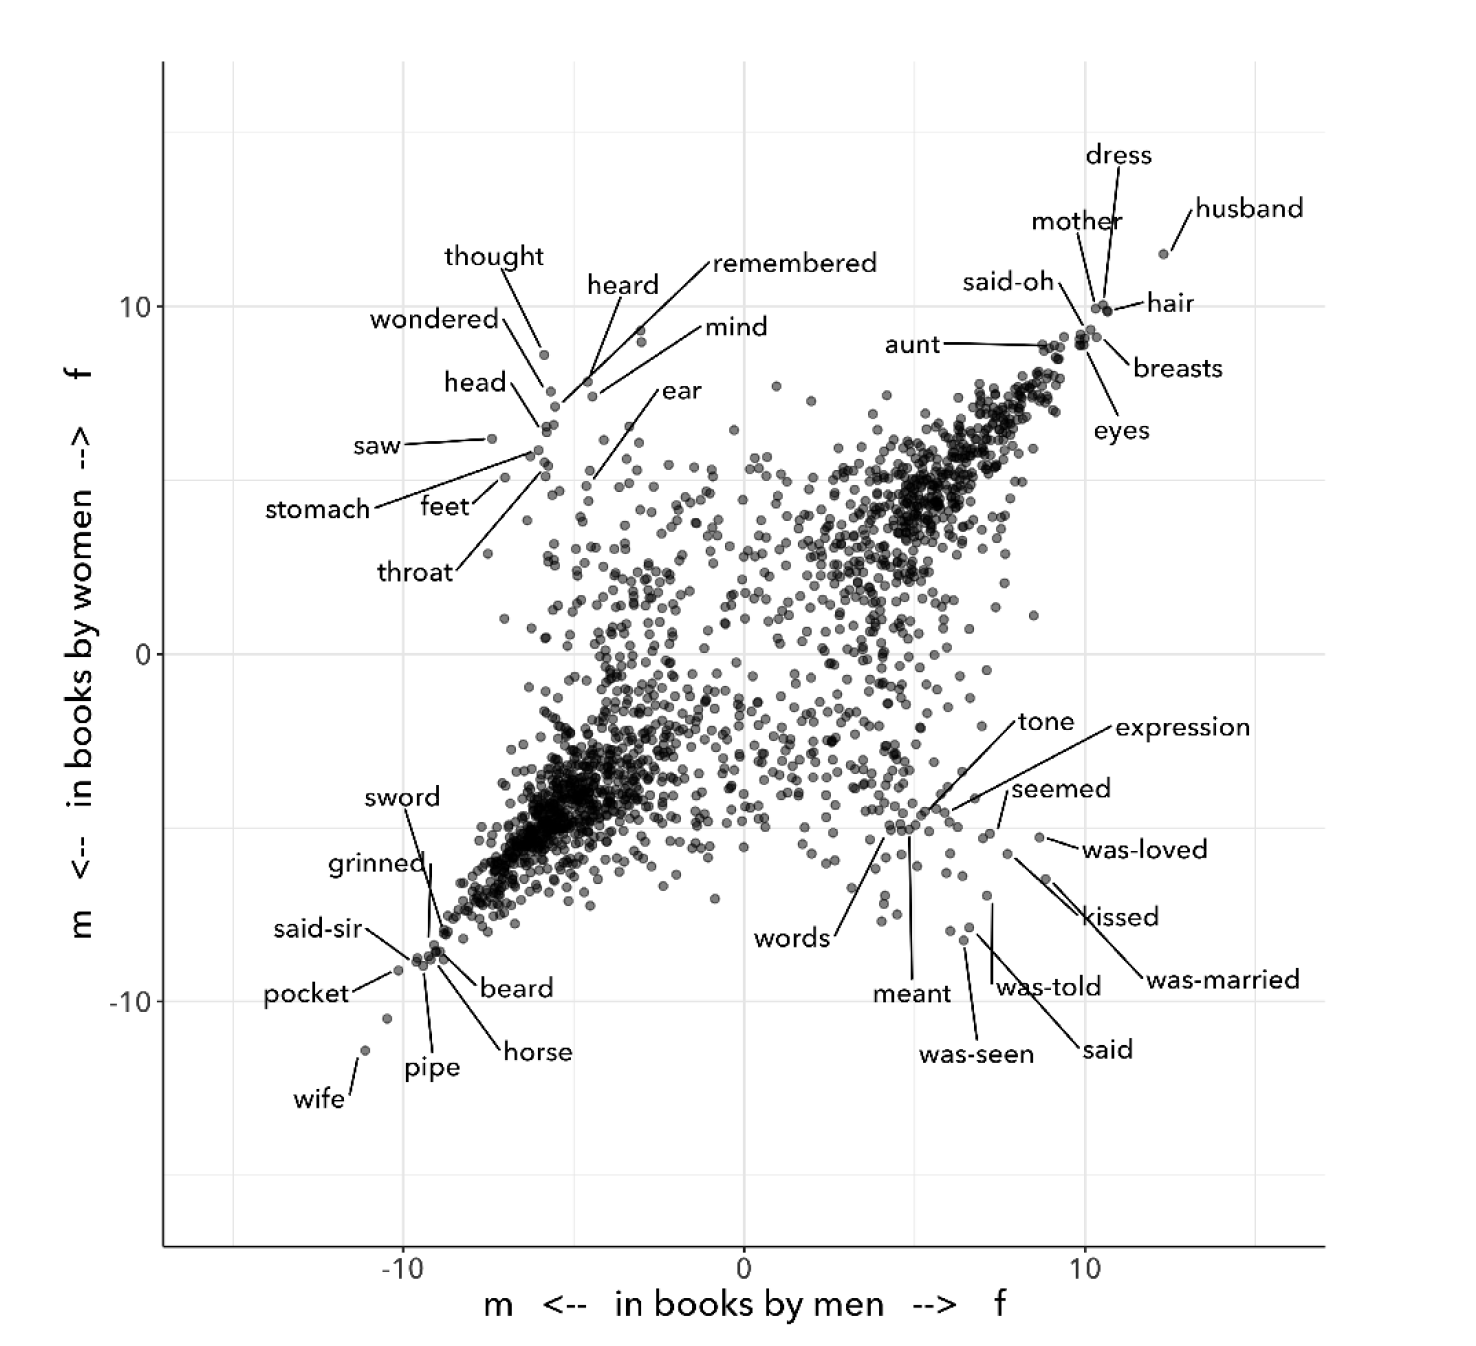
\includegraphics[width=.9\linewidth]{./img/Underwood.png}
\end{center}

There are two important things to point out about Underwood's
analysis. First is that his specific method for text analysis is
logistic regression analysis, which is made for modelling binary
variables. A logistic regression expresses information in the form of
a probability, often between yes/no, pass/fail, win/lose, etc. In
Underwood's case, the probability is male/female. The output therefore
conforms to this binary model. Second, underpinning his methodology,
there is a larger issue with the question that Underwood poses. From a
critical gender perspective, Underwood's question imposes the very
structure that he is attempting to deconstruct. In other project where
he similarly measures the "transformations" of gender across time
periods, he explains that simplification is necessary ("Machine
Learnig and Human Perspective" 93). Underwood admits that he needs a
"simple" model in order to bring into relation the dynamics of gender
(See Fig. 2).\footnote{He measures the "gendering of words used in characterization"
("Machine Learning and Human Perspective" 95), that is, gender
portrayed in novels by women and in novels by men. The verticle axis
visualizes the representation of words by women, and the horizontal by
men, with positive numbers signifying overrepresentation of these
terms. So terms on the top right are words that are used often by men
and women writers, and terms in the upper left and lower right are
ones used most often by women and men, respectively.} He explains:
\begin{quote}
I recognize that gender theorists will be frustrated by the binary
structure of the diagram. To be sure, this binary has folded back on
itself, in order to acknowledge that social systems look different
from different positions in the system. But the diagram does still
reduce the complex reality of gender identification to two public
roles: men and women. I needed a simple picture, frankly, in order to
explain how a quantitative model can be said to represent a
perspective. "Machine Learning" 98
\end{quote}
In aiming for simplicity, Underwood underestimates the extent to which
his initial assumptions will affect the final result. Although he
considers the possibility that he finds a structural tension between
gender "because [he] explores gender, for the most part, as a binary
opposition" (\emph{Distant Horizons} 140), he neglects to consider how the
collapsing of gender into a single graph perpetuates the structural
categories of male/female and the assumptions behind such a
category.\footnote{Add a quote here from Laura Mandell on F/M categories?} The issue is not just with the assumptions at the
outset which reproduce the result, but with the guiding question of
the entire project, which is not about deconstructing gender, but
about reifying it. Asking a machine to replicate the conscription of
gender as male/female for the purpose of seeing how male and female
roles in novels change over time only creates a model of gender that
is "simple" enough to be computed.

How does simplifying the concept of gender contribute to our study of
it? Underwood's "simple" model recalls with what Eve Kosofsky Sedgwick
describes as "a binary mode of thinking," which searches for what
might affirm or deny the point of interrogation. Sedgwick explains
that this process creates a formula for literary analysis by which
reading becomes a mechanical practice of searching for what is hidden
or absent which will finally explain some latent meaning in the text
(Sedgwick Touching Feeling 12). Then, This process is replicated as
the search for meaning takes on other texts, imposing the same
structure on new material. Underwood himself states: "the data I can
legally provide -- lists of word frequencies associated with each
volume or fictional character -- should allow intrepid readers to
retrace the most debatable parts of the argument. An argument that can
be retraced in this manner is 'reproducible'" (Underwood, \emph{Distant
Horizons} 173). He continues, "If my conclusions hold true in
different subsets of the literary past, they are not just reproducible
but 'replicable'" (Underwood, \emph{Distant Horizons} 174).

Laura Mandell explores solutions for approaching the reduction of
gender as data, into what she calls the "M/F binary."\footnote{Mandell, Laura. “Gender and Cultural Analytics: Finding or
Making Stereotypes?” Debates in Digital Humanities 2019. Edited by
Matthew K. Gold and Lauren Klein. University of Minnesota Press, 2019.} Mandell
demonstrates how the M/F binary is reified "by presenting conclusions
about “male” and “female” modes of thinking and writing as if the M/F
terms were simple pointers to an unproblematic reality, transparently
referential and not discursively constituted" (par. 5). Mandell's
examination marshalls key findings from feminist theory, drawing from
Judith Butler, among others, to assert that gender is a socially
constituted category, a "performance" that can be historicized. She
illustrates the guiding power of the M/F binary in her critique of
Matthew Jockers and Jan Rybicki, finding that they essentialize gender
by relying on stereotypes in their premises.\footnote{Jockers, Matthew L. Macroanalysis: Digital methods and literary
history. University of Illinois Press, 2013; Rybicki, Jan. “Vive la
différence: Tracing the (Authorial) Gender Signal by Multivariate
Analysis of Word Frequencies.” Digital Scholarship in the Humanities
(2015): 1–16. doi: 10.1093/llc/fqv023.} Mandell uses
stylometry, as well as word-frequency analysis, and topic modeling to
examine gender in writing.\footnote{Such methods are often used in assessing authorship and
authenticity, and stylometry in particular predates computing and has
notable cases in English Renaissance drama and biblical
texts. Generally, stylometry evaluates writing style by extracting and
analysing distinctive features in text. Often used in stylometry,
word-frequency analysis examines word usage to determine authorship of
a text.} Topic modeling, as explained above,
is the generation of categories or "topics" about text. Mandell uses
the popular stylometry measurement, "Burrow's Delta," which visualizes
the "distance" between writing styles by creating branches (or
"deltas") between different texts. Specifically, Mandell's analysis
focuses on the "most frequent, little words (“a,” “of,” “the”), as
well as keywords."

Mandell suggests that quantitative methods can open up the way we
deconstruct our understanding of quantification and gender. She points
out that gender, which is "constructed both by the measurer and the
measured," is never just about gender, but contains multiple
assumptions. To demonstrate how gender is "constructed," she poses a
counter experiment with genre, which finds that genre analysis cuts
across the gender binary. She comapres the stylistic qualities of a
female writer, Mary Wollenstonecraft, against two male writers,
William Godwin and Samuel Johnson, revealing that: "Wollstonecraft’s
sentimental anti-Jacobin novels most resemble Godwin’s sentimental
anti-Jacobin novels\ldots{} whereas her essays most resemble Johnson’s
writings" (par. 29). Wollenstonecraft's writing resembles both male
and female writing, depending on the genre. To analyze the highly
constructed category of "gender," then, one must also consider genre:
"separating gender from other markings (genre, era of composition) is
not possible: historical time and genre are not incidental to, but
constitutive of, gender" (par. 35).

Admitting the constructed nature of gender allows researchers "to
experiment with new taxonomies of gender" (par. 37). Most usefuly,
Mandell's work points out how the computer is ideal for drawing
attention to the multiplicity of gender. The potential for complex
data models potentially allows researchers to "break the strength of
the signal" in the M/F binary by creating new categories, such as
"'men writing as men,' 'women writing as women,' 'women writing as
men,' 'men writing as women,' 'unspecified (anonymous) writing as
men,'" and so on (par. 35). Moreover, her emphasis on visualization
and movement inform how one might "animate numerical processes rather
than fixing their results as stereotype" (par. 7). The dynamicity of
computation, which allows one to run data iteratively, feeding new
inputs into new results, complicates any straighforward understanding
of the M/F binary. Mandell explains that “Computer screens\ldots{} afford
the fluid exploration of parameters and taxonomies, through which many
sorts of experiments can be tested: interactive visualizations can
give us not objective answers rooted in aggressively reductive
oppositions, but parallax, multiple perspectives for viewing a very
complex reality” (par. 38).

However enlightening Mandell's deconstructive approach, she does
overlook a crucial aspect about gender--that it is highly constitutive
of subjectivity. The similarities that Mandell draws between gender
and genre evacuate how gender is \emph{constitutive} of the
subject. Borrowing from Butler, she argues that both gender and genre
as a performance "are\ldots{} highly imitable" (par. 30), and asserts that
"Anyone can adopt gendered modes of behavior, just as anyone can write
in genres stereotypically labeled M/F" (par.30). Here, she takes
Butler's points about gender as a performance in \emph{Gender Trouble} too
literally. As Butler clarifies in her later work, performativity is a
\emph{process} which is compulsory and habitual, rather than a singular
act. Crucially, Butler asserts that gender \emph{precedes} and
\emph{constitutes} the subject and explicitly warns against the
interpretation that gender is decided by the subject, to be put on and
off at will like clothing. Rather, according to Butler, the subject
\emph{is produced} by gender; gender is more like a mechanism that allows
the subject to emerge: "construction is neither a subject nor its act,
but a process of reiteration by which both 'subjects' and 'acts' come
to appear at all" (\emph{Bodies} xviii). This is not to say that Mandell is
wrong about gender being constructed, but that her assumption, that
"categories such as gender are being constructed both by the measurer
and the measured" misses an important point about the way that gender
constitutes subjectivity (par. 38). According to Butler, the subject
only emerges as an effect of gendered performance. Therefore, to
analyze gender, one might look at the ways that it constitutes and
constrains subjectivity.

I emphasize gender being constitutive because this quality has a
generative parallel to computation. As Mandell points out,
"Computation enables complexity" (par. 36). And computation, like
gender, is also highly constrained, containing rules and protocols
that govern the way that text is processed and analyzed. As So and
Roland demonstrate with the categories of white and black authorship,
the constraints of computation help point out the bounds of social
categories as a constructed phenomenoa. While the work of So and
Roland is essential for bringing together quantitative and critical
race discourses, it also doesn't give enough credit to the ways that
\emph{computers}, in presenting formalized schemas of race, \emph{transform}
data toward speculative ends. Additionally, however, computation might
work within the fram eof speculation. This kind of work would explore
the contraints of gender and computation as \emph{enabling constraints}. As
Underwood acknowledges, computational methods are well suited for
speculative inquiries: "the point of numbers in social science is not
to impose determinism but to acknowledge uncertainty" (Underwood,
\emph{Distant Horizons} 186). If we are going to analyze gender, we might
consider how it constitutes and constrains other elements in the text.


\subsection{Deformance and Performance: NLTK, Gender Trouble, Orlando}
\label{sec:org95a30a2}

This section now turns to the programming language Python to get a
closer look at how text analysis works through constraint. We will
look into the material specificity of text analysis, to examine how it
works, and through what processes and protocols.

Many distant reading projects use a text analysis tool called Python
to do computational analysis of textual data. As a general purpose
programming language, Python is applicable toward many tasks and
projects, from publishing websites, to managing and analyzing large
data sets (of textual and numeric data), to deep learning and
artificial intelligence. The emphasis on readability in Python's code
vocabulary and syntax make it a relatively straightforward programming
language that is easier to pick up than other comparable
languages. Most beginners can jump into the python syntax and intuit a
sense of the code simply by reading it left to right. For example, an
expression called the \texttt{for loop} consists of six words over two lines,
and that instructs Python to do something to each item in a group of
data. In more technical terms, the \texttt{for loop} offers a mechanism for
iterating (or "looping") through data, and carrying out some specified
action to each peice of data. The \texttt{for loop} consists of the following
expression:

\begin{SOURCE}
for letter in "hello":
    print(letter)
\end{SOURCE}

The first line of code specificies the data (\texttt{hello}), and the
second line (\texttt{print(letter)}) instructs the computer to print each
letter in the word. Essentially, this loop will go through each item
in the data, in this case, each letter in the word \texttt{hello}, and it
will \texttt{print} or display that data.\footnote{In JavaScript, for example, the \texttt{for loop} is more convoluted:

\begin{SOURCE}
for (i = 0; i < word.length; i++) \{
  text += word[i] + "<br>";
\} 
\end{SOURCE}} The the output will appear
thus:

\begin{SOURCE}
h
e
l
l
o
\end{SOURCE}

These kinds of iterative computations, which are central to
programming tasks, are a core component of working with text. At a
very basic level, much of text analysis consists of iterating over
bits of text and doing something to each bit. 

A major benefit to a popular programming languages like Python is that
users have developed a number of custom "libraries," or collections of
code for specific tasks like web scraping, data analysis, and text
analysis. In text analysis, there are a number of libraries for
Natural Language Processing (NLP), or the processing of linguistic
data into computational formats. The most popular NLP library in
python is the Natural Language ToolKit (NLTK). This library comes
packaged with a corpus of texts that are ready to analyze, like Herman
Melville's \emph{Moby Dick} (1851) and Jane Austen's \emph{Sense and
Sensibility} (1811). Researchers can use NLTK methods like
\texttt{tokenize()} or \texttt{lemmatize()}, allowing them to process a text from
its oringal format, often a \texttt{string}, or alphanumeric characters in
sequential order, into a "clean" or regularized form. NLTK also
contains useful analytical methods such \texttt{similar()}, which will
generate a list of words that appear in similar contexts to the chosen
word, or \texttt{concordance()}, which will return all the immediate words
surrounding a chosen word. For example, below is a concordance of from
Austen's \emph{Sense and Sensibility} for the word "woman":

\begin{SOURCE}
ties . Had he married a more amiable woman , he might have been made still more
t was so much the greater , and to a woman in Mrs . Dashwood ' s situation , wi
ry comfortable fortune for any young woman ." " To be sure it is ; and , indeed
 way , if he were to wish to marry a woman who had not either a great fortune o
nd of the danger attending any young woman who attempted to DRAW HIM IN ; that 
 to inhabit or visit it while such a woman was its mistress . She instantly wro
income of five hundred a - year by a woman who never saved in her life , they w
as she was a very cheerful agreeable woman , he hoped the young ladies would no
d - humoured , merry , fat , elderly woman , who talked a great deal , seemed v
 should by any chance happen to be a woman who is single at seven and twenty , 
objection to his marrying HER ." " A woman of seven and twenty ," said Marianne
y of a wife . In his marrying such a woman therefore there would be nothing uns
ed Elinor , " to convince you that a woman of seven and twenty could feel for a
ndignity of being approved by such a woman as Lady Middleton and Mrs . Jennings
ch was exactly calculated to carry a woman . Without considering that it was no
been , she had actually made her own woman enquire of Mr . Willoughby ' s groom
ould be attempted . " You are a good woman ," he warmly replied . " Your promis
, he was the husband of a very silly woman ,-- but she knew that this kind of b
 all the philosophy of a well - bred woman , contenting herself with merely giv
rmed at in reality ." " What a sweet woman Lady Middleton is !" said Lucy Steel
 , you cannot tell me what sort of a woman she is ?" " No ," returned Elinor , 
sible he is very capable of making a woman sincerely attached to him ." " Certa
nd I fancy she is an exceeding proud woman ." " I certainly did not seek your c
. Ferrars is a very headstrong proud woman , and in her first fit of anger upon
self - interest alone could induce a woman to keep a man to an engagement , of 
\end{SOURCE}

This tool allows users to examine the context surrounding the chosen
word, "woman." In other words, we see some of the text that comes
immediately before and after the chosen word. This \texttt{concordance}
method is related in its process to another one, \texttt{similar}, which also
uses word context to calculate its output. The result for running
\texttt{similar} on the word "woman" in \emph{Sense and Sensibility} are the
following:

\begin{SOURCE}
man way year moment word men letter friend person gentleman living
situation part lady wife child time thing little day
\end{SOURCE}

To compute terms with \texttt{similar()}, NLTK first takes the context of the
term from \texttt{concordance()}, then it searches the text for other terms
that contain similar contexts. In this sense, the \texttt{similar()} method
searches the text for words that appear \emph{similarly} to the chosen
word. It is a useful strategy for getting a sense of which words are
treated in comaprable ways across the text.


In order to run methods like \texttt{concordance()} and \texttt{similar()}, however,
the text needs to be ready for analysis. This requires a series of
preprocessing tasks like tokenizing, cleaning and regularizing the
text. Tokenizing the text means separating it into units like words
and punctuation. Tokenizing the text transforms a \texttt{string}
(alphanumeric sequence) of characters into workable units, or
\texttt{tokens}, which is easier to clean and regularize. NLTK offers a
method for tokenizing: \texttt{nltk.word\_tokenize()}. Running this method on
the text of Virginia Woolf's \emph{Orlando} turns the novel into a list of
words and punctuation. The following is the first sentence of the
novel in tokenized format:

\begin{SOURCE}
['He', '--', 'for', 'there', 'could', 'be', 'no', 'doubt', 'of',
'his', 'sex', ',', 'though', 'the','fashion', 'of', 'the', 'time',
'did', 'something' 'to', 'disguise', 'it', '--', 'was', 'in','the',
'act', 'of', 'slicing', 'at', 'the', 'head', 'of', 'a', 'Moor',
'which', 'swung', 'from','the', 'rafters', '.' ]
\end{SOURCE}

Once the text is tokenized, then it can be cleaned. Cleaning the text
involves stripping it of capitalized letters and punctuation, such as
"--" and ",", and removing what are called "stop words," or
prepositions, articles, and related terms. In this example, stop words
include "he," "for," "there," "be," "of," "the," and "did."
Punctuation and stop words are often removed because tend to skew or
slow results of analysis due to their high frequency and low semantic
value. Using python's brevity, we can clean and remove punctuation and
capital letters with just one line of code:

\begin{SOURCE}
lower\(_{\text{no}}\)\(_{\text{punct}}\) = [word.lower() for word in tokens if word.isalpha()]
\end{SOURCE}

Reading from left to right, this expression first creates an empty
list, called \texttt{lower\_no\_punct}. Then, for each word in the text, it
makes the word entirely lowercase, and if that word is alphabetic
(meaning it contains no numbers or punctuation), it will be added to
the empty list. Python expressions like this one, which are contained
within brackets on a single line, are called "list comprehensions."
The variable that stores the final data (\texttt{lower\_no\_punct}) is set to a
list comprehension that specifies what to do for each word in the
text. This expression is a kind of condensed loop, which goes through
each item in a list of items (such as each word in a text) and does
something to that item. The same expression can be written in expanded
form by making use of nested structures. For example:

\begin{SOURCE}
lower\(_{\text{no}}\)\(_{\text{punct}}\) = []
for word in tokens:
    if word.isalpha():
        lower\(_{\text{no}}\)\(_{\text{punct.append}}\)(word.lower())
\end{SOURCE}

Here, we begin again by creating an empty list, \texttt{lower\_no\_punct}, into
which we will drop our words after filtering through them. The next
line begins our \texttt{for loop}, which iterates through each word in the
\texttt{tokens} list of words. The third line creates the condition to have
only alphabetic characters in our \texttt{lower\_no\_punct} list. If the word
passes that condition, then we go to the fourth line, which will add
that word to the list. At the same time that this word is added to
this list, all the letters will be transformed to lowercase
format. The final list will contain words that are all lowercase and
contain no punctuation.

Next, we will remove stop words. To do this, we can use another list
comprehension:

\begin{SOURCE}
no\(_{\text{stops}}\) = [word for word in lower\(_{\text{no}}\)\(_{\text{punct}}\) if word not in stops]
\end{SOURCE}

Similarly to the above example, this expression takes each word in a
list, in this case, \texttt{lower\_no\_punct}, and checks to see if that word
is also contained within the list of stop words in \texttt{stops}. If the
word is \emph{not} a stop word, then it will be added to a new list,
\texttt{no\_stops}.  Once this is done, we can take a peek into the first
several words on the cleaned text. We are now left with a list of
words that are all lowercase, without punctuation or stop words:

\begin{SOURCE}
['could', 'doubt', 'sex', 'though', 'fashion', 'time', 'something',
'disguise', 'act', 'slicing','head', 'moor', 'swung', 'rafters']
\end{SOURCE}

After cleaning the text in this way, we can move on to regularization,
which includes lemmatizing. Lematizing is the process of stripping the
grammatical structure to get the word root. In some cases, this
involves cutting off the endings, or affixes, from the word, for
example, "rafters" will be stripped to "rafter." In other cases,
however, it involves looking up a word in a reference to find the
appropriate root. After running the lemmatizer through our text, the
first sentence appears thus:

\begin{SOURCE}
['could', 'doubt', 'sex', 'though', 'fashion', 'time', 'something',
'disguise', 'act', 'slicing','head', 'moor', 'swung', 'rafter']
\end{SOURCE}

There are two aspects about the cleaning and regularizing process that
merit some attention: the first is recursion. The cleaning and
regularizing process is highly recursive, doing the same action to
each item to the list of words that make up the text. The logic of the
code reinforces this recursiveness, especially in the loop which
iterates through items in a list, doing the same thing to each item,
one by one. Additionally, the code's nested expressions reinforce
recursion, as each line specifies another action to be performed on
each word. For example, in the following code block, the first line
isolates a word from the list, the second line checks if that word
contains only alphabetic characters, and the third transforms that
word to lowercase. Each of the three lines performs an additional task
on the same word.

\begin{SOURCE}
for word in tokens:
    if word.isalpha():
        word.lower()
\end{SOURCE}

The second notable aspect about the cleaning and regularizing process
is reduction. These tasks of preprosessing text force words into
existing boxes, so to speak, in order to make them amenable to
analysis. The effect of this preprocessing therefore strips text of
some of its semantic meaning, which can be contained in capitalized
words, rhythms of language in stop words, inflections in word endings,
and so on. That preprocessing potentially strips meaning from words
doesn’t mean that it ought to be avoided, but that the researcher
ought to be aware of how certain textual reductions have the potential
to affect meaning. For example, the novel \emph{Orlando} opens with this
assertive gender designation, followed by an immediate qualification
of this designation, which is expressed entirely in stopwords and
punctuation. The removal of stopwords from the opening sentence strips
the immensely meaningful first word "He," which asserts the gender of
the protagonist. It also cuts the following em dash, which leads to an
interruption that immediately qualifies the previous assertion "--for
there could be no doubt of his sex--." In preprocessing, such details
would be read as semantically void and would be subsequently removed
from the data.

\subsubsection{constraint of gender: queer performantivity}
\label{sec:org57b4f41}
These critics all approach the interaction between reader and text as
a peformative phenomenon. They discuss the event of the analysis,
"playing the text", making "cuts" into the data. By contrast, the
aspect of performativity that gender theorists like Judith Butler
emphasize is that of repetition, signification, and
re-signification. Butler performativity as a repetitive activity,
constrained by regulatory norms, which produces subjects. Although
performativity regulates subjects toward heteronormative practices, it
can also be coopted into subversion. In the process of repetition,
subjects have the possibility of resignifying meaning by producing it
differently. This resignification allows subjects to work within their
limitations to resist dominant structures while maintaining their own
sense of exclusion without being coopted. In other words, they can be
in the system but not of the system.

In her groundbreaking book, \emph{Gender Trouble: Feminism and the
Subversion of Identity} (1990), Judith Butler famously disrupts
popular theorizations about sex and gender in contemporary feminist
thought: namely, that sex is biological while gender is constructed;
and that the gender, as a construction, is a self-expression of the
subject. According to Butler, sex and gender are both social
constructions, and there is no such thing as a stable gender identity,
or even a subject that exists prior to gender expression. Rather,
Butler argues that gender is performative--it is a series of repeated
acts by which the subject enacts gender by "citing" heteronormative
regulatory schemas. It is through the process of enacting gender that
the subject emerges. In her follow up book, \emph{Bodies That Matter}
(1995), Butler further delineates the process of gender
performativity, where what is experienced as the physical body, its
boundaries and its sexuality, only materialize through the repetition
or “citation” of cultural norms. Her concept of "citation" emphasizes
the iterability of the performative practice, whereby each action
"cites" or implicitly signals an authorizing norm. According to
Butler, performance consists of this habit of citation, the ongoing
process of submitting behavior to a regulatory norm.

Here, Butler's central concern is to explore how language and the body
engage. Specifically, Butler wonders whether language can indicate a
body that has not yet been imbued with meaning, a body "prior to
signification" (6). She wonders, "Can language simply refer to
materiality, or is language also the very condition under which
materiality may be said to appear?" (6). Butler finds that language
cannot refer to a pre-existing materiality--for to refer to the body,
language must first posit that body, and in the positing, it assumes
meaning. Therefore, she reason, the signification of the body actually
creates the body: "This signification produces as an \emph{effect} of its
own procedure the very body that it nevertheless and simultaneously
claims to discover as that which \emph{precedes} its own action"
(6). Language, rather than reflect a prior reality, actually works to
\emph{produce} signification. Butler's point here draws from feminst
theorist Luce Irigaray who argues that language in fact creates
knowledge, as in her famous statement about female sexuality, which
"has always been conceptualized on the basis of masculine parameters"
(Irigaray, \emph{The Sex Which Is Not One} 23). Butler points out that "the
mimetic or representational status of language\ldots{}. is not mimetic at
all. On the contrary, it is productive, constitutive, one might even
argue performative" (6). In other words, language produces the reality
that it claims to merely reference. So, in the process of citation,
which is the ongoing re-signification that cites regulatory norms such
as gender norms, subjects are always interpellated by a discourse
prior to their citing it. This productive quality of language will be
central to the ways that language offers a way out of the
significatory circle.

Butler asks, "What would it mean to cite a law to produce it
differently, to 'cite' the law in order to reiterate and coopt its
power?" (xxiii). For, amid this regulatory structure, in which the
subject comes into being by continually citing the norm, lies the
possibility of resignifying that citation. Because language transcends
a representative function, because it has the ability to \emph{produce}
meaning, language can be resignified toward subversive usages by
\emph{citing the repudiated signification}. Butler offers an example in the
resignification of the term "queer," which has been transformed from a
term of abjection to one of empowerment. "Queer" achieves this
signification by harnessing its own repudiation, which Butler explains
is implied by every identification, a "disavowed abjection [which]
will threaten to expose the self-grounding presumptions of the sexed
subject" (3). By identifying with heterosexuality, one repudiates
homosexuality, the "Queer," which will remain as a threat to the
identification. Butler proposes that one marshall this repudiation as
a resource in resignification: "to consider this threat and
disruption\ldots{} as a critical resource in the struggle to articulate the
very terms of symbolic legitimacy and intelligibility" (3). Here, the
concept of "citation" is crucial, for each signification "cites" or
draws from the authorizing power. One can cite a norm in order to
disrupt the significatory power of that norm. So, the term "queer," in
its public assertion, "enacts performativity as citationality for the
purposes of resignifying the abjection of homosexuality into defiance
and legitimacy" (xxviii). Each time the term is used, it draws from
the domain of abjection, the repudiation, in a way that re-signifies
because it fails to repeat the meaning loyally, because it signifies
that meaning differently. For Butler, then, the central problem of
being stuck in the cycle of signification is also the solution. Butler
takes on language as something that can be productive, that can
resignify meaning, as the option available to those who are trapped
within the signification system.

An exploration of Luce Irigaray's writing style demonstrates how this
process of resignification can take place in language. First, Butler
establishes how significatory systems exclude that which they claim to
signify. Irigaray takes Jacques Derrida's concept of phallogocentrism,
or that man, symbolized by the phallus, is the center and focus of
knowledge, as a lens for reading Plato and Aristotle's discussion of
form/matter or bodies/souls binaries. Irigaray demonstrates how these
binaries, which take the category of "woman," associated with "matter"
(materiality, the mother) and set it subordinate to male "form"
(mastering rationality) actually erase the possibility of representing
woman at all. In fact, the binary that claims to represent the
feminine as the subordinated term in masculine/feminine binaries,
actually "produces the feminine as that which must be excluded for
that economy to operate" (10). Because "binary oppositions are
formulated through the exclusion of a field of disruptive
possibilities"(10), the feminine is "domesticated" (13). The
nonfigured feminine remains excessive, outside the terms of the
binary:
\begin{quote}
One cannot interpret the philosophical relation to the feminine
through the figures that philosophy provides, but, rather, she argues,
through siting the feminine as the unspeakable condition of
figuration, as that which, in fact, can never be figured within the
terms of philosophy proper, but whose exclusion from that propriety is
its enabling condition. 12
\end{quote}
What Butler calls the \emph{excessive} feminine is excluded, or cast out,
as "the necessary outside," which allows the \emph{specular} feminine to
take its place in the binary. According to Butler, we cannot know what
the feminine consists of without subscribing it to
phallogocentrism. If the feminine is outside the system, and cannot be
figured, how can it be known? Butler aptly questions, "For how can one
read a text for what does \emph{not} appear within its own terms, but which
nevertheless constitutes the illegible conditions of its own
legibility?" (11). For Butler, this is the key question--how do we
work with what we are given to express what is not there, what is
refused by the system of the visible?

The answer is through repetition and reworking--resignification
through performative citation. Butler explains that Irigaray achieves
this resignification by miming language: "she mimes philosophy\ldots{} and,
in the mime, takes on a language that effectively cannot belong to
her" (12). Butler reads Irigaray's use citation as a strategy of
repeating what Plato says with the goal of undermining his authority:
"She cites Plato again and again, but the citations expose precisely
what is excluded from them, and seek to show and to reintroduce the
excluded into the system itself" (18). Through repetition, Irigaray
displaces the logic of phallogocentrism, introducing something
external to the system while remaining within its terminology. Butler
affirms that "Her miming has the effect of repeating the origin only
to displace that origin as an origin" (18). Her repetition is a way of
infiltrating the logic of phallogocentrism on its own terms. Butler
herself mimes what might have been Irigaray's internal monologue:
\begin{quote}
I will not be a poor copy in your system, but I will resemble you
nevertheless by miming the textual passages through which you
construct your system and showing that what cannot enter it is already
inside it (as its necessary outside), and I will mime and repeat the
gestures of your operation until this emergence of the outside within
the system calls into question its systematic closure and its
pretension to be self-grounding" (18).
\end{quote}
Deception through resemblance; insubordination through subservience;
displacement through repetition--these are the tools available to the
subject that remains outside the logic of phallogocentrism.

\subsubsection{orlando close reading - gender as enabling constraint}
\label{sec:org8f90aaf}
As I previously examined NLTK for how it guides and constrains
analysis, I now turn to looking at \emph{gender as a constraint} in
Virginia Woolf's novel, \emph{Orlando: A Biography}. In what follows, I
will demonstrate how gender functions as an \emph{enabling constraint} in
Virginia Woolf's text, \emph{Orlando: A Biography}, to examine how the
phenomenon of gender guides and influences subjectivity.

\emph{Orlando} is a fictional biography that follows the life of the
eponymous 16th-century English nobleman as he undergoes a sex change
and lives into the 20th century as a woman. In this text, gender is
linked to the role of language in the way that they both activate
significatory power. My reading explores how the beginning of the
novel displays the common struggle between gender and language for for
expression. I then point out key moments where the novel approaches
gender through the prism of language, specifically in the tension
between plain language and poetic language as experienced by Orlando
as he develops into a poet and by the biographer-narrator, who
repeatedly disclaims literary and figurative strategies of narration
while striving for an objective portrayal of Orlando's life. Then, I
show how Orlando's sex change begins to resolve his struggle with
language, and therefore, gender. As Orlando settles into her new
gender, she finds new significatory power in language. At the same
time, the biographer is freed to explore more experimental forms for
telling Orlando's story.

At the beginning of the story, Orlando falls in love with a young
Russian princess named Sasha. The scene of this romance is an
important moment where gender is explored in relation to language,
because Orlando cannot resolve either one. When he first sees Sasha,
she is skating over the frozen river Thames, and he cannot ascertain
if she is a man or a woman from her skilled atheleticism and exotic
manner of dress. He proceeds to describe her using seemingly arbitrary
metaphors--another significatory attempt that also fails:
\begin{quote}
He beheld, coming from the pavilion of the Muscovite Embassy, a
figure, which, whether boy's or woman's, for the loose tunic and
trousers of the Russian fashion served to disguise the sex, filled him
with the highest curiosity. The person, whatever the name or sex, was
about middle height, very slenderly fashioned, and dressed entirely in
oyster-coloured velvet, trimmed with some unfamiliar greenish-coloured
fur. But these details were obscured by the extraordinary
seductiveness which issued from the whole person. Images, metaphors of
the most extreme and extravagant twined and twisted in his mind. He
called her a melon, a pineapple, an olive tree, an emerald, and a fox
in the snow all in the space of three seconds; he did not know whether
he had heard her, tasted her, seen her, or all three together. (For
though we must pause not a moment in the narrative we may here hastily
note that all his images at this time were simple in the extreme to
match his senses and were mostly taken from things he had liked the
taste of as a boy. But if his senses were simple they were at the same
time extremely strong. To pause therefore and seek the reasons of
things is out of the question.)\ldots{} A melon, an emerald, a fox in the
snow--so he raved, so he stared. When the boy, for alas, a boy it must
be--no woman could skate with such speed and vigour--swept almost on
tiptoe past him, Orlando was ready to tear his hair with vexation that
the person was of his own sex, and thus all embraces were out of the
question. 
\end{quote}
This passage expresses a mounting sense of tension as Orlando grows
more and more frustrated with Sasha's gender ambiguity. Interestingly,
his growing frustration seems to feed his attraction, as with each
doubt Orlando appears more and more desperate, "ready to tear his hair
with vexation." The biographer's role in the narrative unfolding of
this scene also has an effect: the syntax alternates long and short
sentences in a way that draws out the cyclical quality of Orlando's
confused mental state. There is also a "pause" in the action, where
the biographer adds another layer of speculation to Orlando's already
conflicted inner life, while simultaneously drawing attention to the
constructed quality of the narrative. While the tension is mounting
throughout the passage, the relationship between gender and language
come to the fore. The biographer's aside, which describes how the
difficulty of placing gender emerges in the difficulty with language--
"He called her a melon, a pineapple, an olive tree, an
emerald"--emphasizes the connection between gender and the
imagination. Intrestingly, at the same time that Orlando cannot place
Sasha's gender, he also cannot find the right words to describe
her. As the Sasha's probable gender oscillates between male and female
throughout passage, and Orlando's desire crescendos, gender seems
primed to signify imaginative beyond biological species, nevermind
sex. The effect of the narrative style in this section is to mirror
with language the tortuous thought process that Orlando undergoes as
he guesses then doubts the reality of Sasha's gender. As the passage
continues, the suspense comes to a climax:
\begin{quote}
But the skater came closer. Legs, hands, carriage, were a
boy's, but no boy ever had a mouth like that; no boy had those
breasts; no boy had eyes which looked as if they had been fished from
the bottom of the sea. Finally, coming to a stop and sweeping a
curtsey with the utmost grace to the King, who was shuffling past on
the arm of some Lord-in-waiting, the unknown skater came to a
standstill. She was not a handsbreadth off. She was a woman. 27-28
\end{quote}
Again, this narrative structure reinforces Orlando's ambivalence about
Sasha's gender ambiguity. The sentences ebb and flow as Orlando
finally settles on Sasha's gender--"she was a woman." Gender is an
element that functions within the story, as something that Orlando
struggles to grasp, in this case, with language. The biographer's
narrative style here, which depicts Orlando's struggle with gender via
langauge, add another layer of language experimentation in the form of
his narrative style. This scene scene shows how if gender is
ambiguous, then language is also imprecise.


As Orlando's relationship with Sasha ends with deceit and desertion,
he succumbs to a long, deep depression that brings him to doubt both
what he had previously been most moved by: love and poetry--"Thys, at
the age of thirty, or thereabouts, this young Nobleman had not only
had every experience that life has to offer, but had seen the
worthlessness of them all. Love and ambition, women and poets were all
equally vain. Literature was a farce" (71). At this time, Orlando
begins to doubt language's ability to convey truth. In one scene, he
struggles both with objective or "plain" language, and with poetic
language, by attempting to describe the color of the grass and the
sky:
\begin{quote}
'The sky is blue,' he said, 'the grass is green.' Looking up, he saw
that, on the contrary, the sky is like the veils which a thousand
Madonnas have let fall from their hair; and the grass fleets and
darkens like a flight of girls fleeing the embraces of hairy satyrs
from enchanted woods. 'Upon my word,' he said (for he had fallen into
the bad habit of speaking aloud), 'I don't see that one's more true
than another. Both are utterly false.' And he despaired of being able
to solve the problem of what poetry is and what truth is and fell into
a deep dejection. 75
\end{quote}
Orlando cannot comprehend whether plain english, where he can say
simply that "the sky is blue; the grass is green" is preferable to a
more figurative language, which makes use of similitude and allusion:
"the sky is like the veils which a thousand Madonnas have let fall
from their hair; the grass fleets and darkens like a flight of girls
fleeing the embraces of hairy satyrs from enchanted woods". For
Orlando, both plain and figurative language appear deficient. At this
point in the story, he has lost his faith in the power of language to
signify. 

The struggle with language operates at two levels across the story: At
the same time that Orlando has his doubts about language, so the
biographer grapples with his narrative project. At the start of the
story, the biographer mocks the techniques of historical biographers
by continualling calling into question the ability of language to
adequately describe life. An early passage begins with the narrator
noting Orlando's exquisite beauty: "A more candid, sullen face it
would be impossible to find. Happy the mother who bears, happier still
the biographer who records the life of such a one! Never need she vex
herself, nor he invoke the help of novelist or poet" (12). From the
beginning, the text displays the biographer's ambivalence about how to
describe Orlando and presents two possible perspectives--that of the
poet, and that of the biographer.The biographer asserts his aims are
to record Orlando as a scribe, "following after" him, "from deed to
deed, from glory to glory, from office to office" (12). But then, as the
passage progresses, the narrator relies on figuration:
\begin{quote}
The red of the cheeks was covered with peach down; the down on
the lips was only a little thicker than the down on the cheeks. The
lips themselves were short and slightly drawn back over teeth of an
exquisite and almond whiteness. Nothing disturbed the arrowy nose in
its short, tense flight; the hair was dark, the ears small, and fitted
closely to the head. But [..] directly we glance at Orlando standing
by the window, we must admit that he had eyes like drenched violets,
so large that the water seemed to have brimmed in them and widened
them; and a brow like the swelling of a marble dome pressed between
the two blank medallions which were his temples. Directly we glance at
eyes and forehead, thus do we rhapsodize. Directly we glance at eyes
and forehead, we have to admit a thousand disagreeables which it is
the aim of every good biographer to ignore. 12-13
\end{quote}
Honoring his committment for straightforward narration, the
description of Orlando's face begins soberly enough with simple
sentence structure that describe Orlando's features with some
insertion of modest figurative comparisons (the "peach down" ob the
lips, teeth of "an exquisite and almond whiteness," the "tense flight"
of the "arrowy nose," etc). However, when the biographer arrives to
Orlando's eyes and forehead, his style ascends into full-fledged
figuration, admitting Orlando has eyes "like drench'd violets." The
biographer's problem, that Orlando is too beautiful for literal
description requires him to draw on the strategies of the poet, using
imagery and simile. Further in the story, in the chapter of Orlando's
sex change, the biographer again falls back onto poetic strategies to
tell Orlando's story. The biographer begins this chapter by laying out
the challenge of describing Orlando's life in a way that is objective
and literal, in keeping with the principles of biography. As he tries
to piece together the events of Orlando's sex change, the biographer
explains that the record of Orlando’s life during this period is
incomplete, because a fire broke out and destroyed much of the
evidence: "Just when we thought to elucidate a secret that has puzzled
historians for a hundred years, there was a hole in the manuscript big
enough to put your finger through\ldots{} often it has been necessary to
speculate, to surmise, and even to use the imagination" (88). The
biographer explains that he must work from fragments, and that his
work involves the use of speculation, much like a 

Orlando's relationship to language begins to change as she transitions
from male to female. The relationship to language begins with the
narrator, who is the first to assert the change in gender pronouns:
\begin{quote}
We may take advantage of this pause in the narrative to make certain
statements. Orlando had become a woman--there is no denying it. Bu tin
every other respect, Orlando remained precisely as he had been. The
change of sex, though it altered their future, did nothing whatever to
alter their identity. Their faces remained, as their portraits prove,
practically the same. His memory--but in future, we must for
convention's sake, say 'her' for 'his;' and 'she' for 'he'--her memory
then, went back through all the events of her past life without
encountering any obstacle. 102-103
\end{quote}
Here, the narrator cycles through the pronouns "he," "they," "she," in
a way that shows how language lags behind gender. The biographer's
language is catching up to the reality of Orlando's new gender. This
is an example, quite literal, of how language struggles to represent
gender, how it is just behind the expression of gender.

After the sex change, Orlando meets and marries a gender ambiguous man
named Shel. As Orlando falls in love with Shel, her issues with
language begin to resolve. She has an experience where language
suddenly takes on significatory power. In a scene that revises a prior
one of the young, heartbroken Orlando attempting to describe the color
of the sky and the grass, Orlando is now in Hyde Park, watching a toy
boat negotiate a wavelet on the Serpentine river. Momentarily, the
boat is dissapears then re-emerges on the other side of the
wavelet. Suddenly associating this moment with the word "ecstasy,"
Orlando hurries to telegram the phrase, 'a toy boat on the serpentine'
and 'ecstasy,' to Shel, who she knows will immediately understand what
it means. As she goes to the post office, she meditates on the nature
of language and literature, which she now realizes is violently
ecstatic.
\begin{quote}
'A toy boat, a toy boat, a toy boat,' she repeated, thus enforcing upon
herself the fact that it is not articles by Nick Greene on John Donne nor
eight-hour bills nor covenants nor factory acts that matter; it's
something useless, sudden, violent; something that costs a life; red,
blue, purple; a spirit; a splash; like those hyacinths (she was passing a
fine bed of them); free from taint, dependence, soilure of humanity or
care for one's kind; something rash, ridiculous, like my hyacinth,
husband I mean, Bonthrop: that's what it is--a toy boat on the
Serpentine, ecstasy--it's ecstasy that matters. 
\end{quote}
Unlike the grass and sky from the previous scene, language now has the
power to signify. "A toy boat" and "ecstasy" are reduced to the same
meaning, a common denominator of feeling. This reduction elevates the
potential for language to capture and convey meaning. The symmetry of
these two episodes shows how Orlando moves beyond a disappointment in
the limitations of language for expression to a new faith in its power
to mean.

As Orlando resolves her struggle with language, so does the
biographer. As the story progresses, the biographer increasingly drops
his pretension toward accuracy and boldly speculates, without excuses,
elements of the story. At one point, when Orlando first meets her
lover Shel, the biographer draws the reader into this
speculation. Shel is a ship captain who exhibits as many feminine
qualities as Orlando does masculine. The biographer describes a scene
of their early courtship:
\begin{quote}
'Shel, my darling,' she began again, 'tell me\ldots{}' and so they talked
two hours or more, perhaps about Cape Horn, perhaps not, and really it
would profit little to write down what they said, for they knew each
other so well that they could say anything, which is tantamount to
saying nothing, or saying such stupid, prosy things as how to cook an
omelette, or where to buy the best boots in London, things which have
no lustre taken from their setting, yet are positively of amazing
beauty within it. For it has come about, by the wise economy of
nature, that our modern spirit can almost dispense with language; the
commonest expressions do, since no expressions do; hence the most
ordinary conversation is often the most poetic, and the most poetic is
precisely that which cannot be written down. For which reasons we
leave a great blank here, which must be taken to indicate that the
space is filled to repletion.
\end{quote}
The biographer here explains that, though it was actually beautiful
and poetic when it took place, this conversation would come across as
extremely ordinary and boring to the reader. An ordinary conversation
can be poetic at the moment of expression, delivered or said in a way
that is beautiful, which may then lose in language. The reader then
encounters a space break which the biographer instructs her to imagine
is "filled to repletion." This space break recalls the episode with
the manuscript, where the biographer points out that there are holes
or gaps in the record. However, while previously there was a problem
with evidence, now it is a problem with language. According to the
biographer, the means to express this conversation doesn’t exist in
language. As a result, the biographer invites the reader to fill in
the space. To use speculation and guesses as to what happened. The
reader must do what the biographer did when he confronted the lack of
evidence, which was to guess what happens from the available evidence.

In troubling the line between objective reality and subjective
experience, Woolf’s parodic biography explores how language and gender
are similarly (and coordinately) constructed. This development in
language both within the story and on the level of narration is
coordinated with Orlando's gender development. Comparing the
biographer and Orlando's experiences with language surface an
interesting insight: language and gender are connected because they
both contain significatory power. While earlier in the novel, Orlando
cannot express the meaning of "blue" and "green," she resolves the
significatory power in the phrase "toy boat." At the same time, at the
level of narrative perspective, the biographer also resolves his issue
with a lack of evidence in the space break that breaks open language's
ability to mean. Language and gender are connected by using the
imagination in creating significatory power, constructing meaning. The
difficulty with language that Orlando and the biographer both
experience becomes less and less of an issue as Orlando comes into her
femininity, which is to say, becomes comfortable in herself. These
changes are possible because the narrative embraces the influence of
the imaginary in language, in minding meaning in words and in
storytelling. This allows Orlando to accept the role of the
imagination in gender, in making gender meaningful.

Later in this chapter, I will use text analysis to further explore the
relationship between these themes: language, gender, and the
imagination. So the question then becomes: how are language and gender
co-constructed in Orlando?  What is the role of the imagination in
gender/language? What is the relation between gender, language, and
the imagination?


\subsection{{\bfseries\sffamily TODO} Queer Distant Reading}
\label{sec:orgf05d4d4}
A method of distant reading attends to gender as an iterative
practice. We find ever expanding ways that gender is characterized in
\emph{Orlando}.

\subsubsection{reproducibility vs iteration}
\label{sec:orgd7194d3}
This notion of iteration--which cuts across both text analysis methods
with NLTK and Butler's theory of gender performativity--is the key for
understanding how a repetitive action can lead to new output. In my
previous discussion of reproducibility, I explain how Underwood's
analysis on gender differences reproduces his assumptions about gender
dynamics as oppositional, as he readily admits: "this chapter has
discovered stable 'structural positions' only because it explores
gender, for the most part, as a binary opposition" (\emph{Distant Horizons}
140). The the binary structure, which is inherent to linear regression
models, reproduces itself the initial assumptions in the
result. Because reproducibility aims for what Underwood describes as a
"simple picture," it collapses or flattens the complexity of data, in
this case, gender, into workable units ("Machine Learning" 98). By
shifting the understanding of reproducibility to iteration, we open up
the possibility for using these tools to interpret elements of gender
and sexuality in text.

\subsubsection{bode and butler parallel on productivity in iteration}
\label{sec:orgb2ff8bf}
Iteration departs from reproducibility because iteration
self-consciously harnesses the productive qualities of
reproducibility. We begin to see this in the way that Bode describes
her critical approach, "agential realism," which mirrors Butler's
explanation of gender performativity. Bode describes two approaches
for literary criticism, the "representationalist" approach (in which
data represents or expresses real objects and subjects in the world)
and the another approach understands data "as part of the ongoing
materialisation of literary texts, as emerging events always arising
from an altering how the literary past as reconfigured" (Bode
"Computational Modeling: From Data Representation to Performative
Materiality"). Similarly, Butler distinguishes a representationalist
approach toward language and materiality, in which language can
\emph{refer} to materiality as something that is prior, against the
performative approach, by which language works through repetition to
signify and resignify meaning:
\begin{quote}
If the body signified as prior to signifiation is an effect of
signification, then the mimetic or representational status of
language, which claims that signs follow bodies as their necessary
mirrors, is not mimetic at all. On the contrary, it is productive,
constitutive, one might even argue performative, inasmuch as this
signifying act delimits and contours the body that it then claims to
find prior to any and all signifcation. Butler 6
\end{quote}
The alignment here between Bode and Butler indicates an intersection
between the digital and gender as processes, which center on the role
of iteration in conveying meaning. There is something fundamentally
productive about these phenomena, and not in the way that they purport
to represent some real quality or object in the world. Rather, the
productive aspect has to do with how they iterate their material over
and again in ways that are fundamentally creative.

\subsubsection{similar\(_{\text{words}}\)("woman" \& "man")}
\label{sec:org5289d51}

In what follows, I will use the python text analysis library NLTK to
analyze gender in Woolf's novel, \emph{Orlando}. Specifically, I will
explore the words associated with "woman" and "man" across this text,
toward the goal of making a kind of "model" for gender performativity
in \emph{Orlando}. Thinking back to my close reading of \emph{Orlando}, I found
that the way that gender works is closely tied to the way that
language works--Orlando and the biographer conflate the difficulty of
expressing gender to that of telling a story, or writing a poem,
thoughout the text. There is something about gender and language which
is highly constrained, as both Orlando and the narrator are oppressed
by them, but also highly imaginative, eventually allowing both
subjects the potential for signification. Therefore, I will begin my
text analysis by exploring how the terms "woman" and "man" are
characterize in the novel. The computational process that I use will
draw from Butler's theory of performativity by "resignifying" the
terms "woman" and "man" in repeated computations. The final output
will present a series of terms associated with man and woman after
various reiterative computations of the terms throughout the text.

We begin by running the \texttt{similar\_words()} method from the
nltk.text.ContextIndex class, which functions very nearly like the
\texttt{Text.similar()} method described previously. This \texttt{similar\_words()}
method takes a word, such as "woman," and returns the top words that
appear most similarly to that word in the text. Below is the
definition of the ContextIndex class from the NLTK source code:

\begin{SOURCE}
class ContextIndex(object):
    """
    A bidirectional index between words and their 'contexts' in a text.
    The context of a word is usually defined to be the words that occur
    in a fixed window around the word; but other definitions may also
    be used by providing a custom context function.
    """
\end{SOURCE}

The NLTK documentation explains that similarity is computed by
processing the words that directly surround the given word, or its
"context," and finding other words that have similar contexts. In the
source code for the \texttt{similar\_words()} method, there is an \texttt{if loop}
that instructs the program to search if the words in the context also
are associated with other words throughout the text. It then returns a
list of the 20 most frequent terms which have similar contexts to the
given word.\footnote{NLTK.text.ContextIndex \url{https://github.com/nltk/nltk/blob/develop/nltk/text.py}}

Below is the output for the words, "woman" and "man," respectively:

\begin{quote}
> similar\(_{\text{words}}\)("woman")
'reached till friend word moment saw always could cried sailor wit
scarcely petticoat go servant conclusion'

> similar\(_{\text{words}}\)("man") 
'hurry father window tongue carriage still even countrywoman indulged
old fortune title ship writing fell become always love grown never'
\end{quote}

\subsubsection{iterating over code resignifies it}
\label{sec:org3efd3af}
Each time a text is processed in computation, it is submitted to a
governing code. In this case of the \texttt{similar\_words()} method, the code
reduces the text to whatever conditions are contained within the
function loop. The output therefore is directly constrained to the
conditions in the input. Each time one feeds the output of our
computation to a new one, running \texttt{similar\_words()} method again, they
gain an even more refined list of words that are associated with
"woman" and "man."  Below are the results of running \texttt{similar\_words()}
taking the output of the previous run of \texttt{similar\_words("woman")} as
the new input:

\begin{SOURCE}
'come friend scarcely make happiness could say wisdom used thing grown
love shape dog wit saw always explain understood ran time prophet
indeed word stood met laughing sailor none able mixture allied woman
fly way year bird might known man toss sake thought reached cried
leave till account first petticoat fool would roused encumbrance
become window rust another madam london'
\end{SOURCE}

And the output for \texttt{similar\_words("man")}, running it a second time:

\begin{SOURCE}
'title come need fault carriage tongue fortune death hungry passion
gloomy grown love written still must always saw exactly alone almost
perhaps take word matter determined orlando beautiful hear hurry woman
boy plump sens man soon little morning full strength whose two father
monstrously without ever would roused kinsman admit become old window
sink moment'
\end{SOURCE}

One may continue to run this \texttt{similar\_words()} analysis, feeding the
output as new input, to get an ever expanding sense of words which are
associated with gender. This would be interesting, as the repertoire
for "woman" and "man" would swell to significations that elude the
gender as a binary. Eventually, however, the repertoire would include
more and more shared terms between the two genders. To avoid what
would inevitably be a merging of words associated with each gender, we
can slightly change the input before running the computation again. We
will filter out any words that were shared between the categories of
"woman" and "man". This will allow us to get a better sense of gender
\emph{distinction} in the text.

Filtering out shared words, and placed unique, similar words for "man"
and for "woman" into a new list, we can run \texttt{similar\_words()}
again. For \texttt{similar\_words()} on the words associated with "woman," we
get the following \emph{unique} words:

\begin{SOURCE}
'among slipping launched child beneath shape new gently prophet indeed
true knee denied fasten bird hot found finger person bred leave nail
reflection character hid used month profit green since ran spoke omit
standing prayer bald frequent good heard scramble try bethink burst
ring street none may happiness wisdom let draw sawings top summer day
upstairs went ribbon known catching case thought ask flung fool voyage
observed minute able people come ala raising gave laughing looked
third side allied fly might slept suddenly thousand going blackness
groping rust sag london'
\end{SOURCE}

For "man," we get:

\begin{SOURCE}
'certain need fault wicket agitate hungry long passion talk circle
ague whatever written turn said explain treachery husband beast
remembered sleep longer pared filled tell princess deep beard tied
beautiful hear put mixture profound fumbled inborn rout immovable
plump awkwardness sens sofa whole mind morning imagine toss many made
iron blush round set whose raised first part monstrously without
needing taste story boyish admitted longed insisted looking glance
pushing'
\end{SOURCE}

By filtering out shared words between "woman" and "man," we come
closer to modelling gender distinctiveness in this text. To be clear,
gender in this sense descends from a binary system--from the initial
analysis of "woman" and "man." However, from this initial
binarization, it leads to a plurality of significations.  

This kind of iterative analysis, where the data is being adjusted to
increase the distinctiveness and complexity of the output, works
toward \emph{resignifying} the initial understanding of "woman" and "man."
It takes what Butler says about gender being an iterative performance,
which is continually "citing" the regulatory norm, and submits this
performance to the highly iterative process of running text through
computational analysis. 

Like gender subversion, this kind of computational analysis works
through strict protocols of repetition and iteration toward some kind
of disruptive end goal. As Alexander Galloway affirms, “Protocol is
synonymous with possibility” (167). Galloway here is discussing
network theory, and by "protocol," he refers specifically to the codes
that append data which mades connections possible in a network. Like
gender performativity, networks are constrained by protocols, which
enable and structure connections between nodes. Despite the
restrictions of protocol, however, there is a freedom in the
possibility of connection, where each node is free to connect to
another within the system.\footnote{Chun, Wendy, \emph{Control and Freedom: Power and Paranoia in the
Age of Fiber Optics}, 2006. Print.} Similarly to hackers in a network,
Butler's idea of gender subversion is is looking for the "exploit,"
the way to disrupt the system by using the system’s own rules. The key
to Butler's exploit is the iterative nature of gender performativity,
which can be used to repeat and resignify meaning.
\begin{quote}
The compulsion to repeat an injury is not necessarily the compulsion
to repeat the injury in the same way or to stay fully within the
traumatic orbit of that injury. The force of repetition in language
may be the paradoxical condition by which a certain agency---not
linked to a fiction of the ego as master of circumstance---is derived
from the impossibility of choice. 83 
\end{quote}
Butler explains that the repetition of language is what enables
a certain agency to emerge in repetition. Repetition is the means by
which dominant or established meaning can be resignified. 

\subsubsection{{\bfseries\sffamily TODO} Findings: new configurations of gender}
\label{sec:orgc9efde6}
\url{https://github.com/rafadavis/intro\_net\_analysis/blob/master/1\_intro.md}

[Visualization of gender distinctiveness in \emph{Orlando} using the python
networkx module]

This [forthcoming!] model of gender distinctiveness in \emph{Orlando} draws
from the same principles as Pamela Caughie et al. in their work in
visualizing gender ontology in \emph{Man Into Woman} (1931), the life
narrative of Lili Elbe, one of the first persons to undergo gender
affirmation surgery. As Caughie and her team struggle to mark gender
shifts throughout the text in a way that accords with the constraints
of the archival methodology, they wonder whether computational models
can capture such taxonomic chaos of gender ontology. However, they
ultimately find that the issue with categorizing gender doesn't need a
solution. Rather, it needs a way of showing gender dynamicity while
still being readable. The scholars point out that the issue with
ontology \emph{should} remain unresolved: "Confusion in gender and sexual
terminologies\ldots{} is part of the experienceof gender and sexuality in
the modernist era, something to be realized and negotiated in readings
of the narrative" (239). Thus they ended up creating a "storm cloud"
of gender, showing clusters of different gender traits in the text
over time.

\subsubsection{{\bfseries\sffamily TODO} the constraint: the power of the imagination}
\label{sec:org99ece71}

In my previous close reading of \emph{Orlando}, I found that gender is
linked to the role of language in the way that they both are highly
constructed phenomena that activate significatory power. After
exploring the ways that gender and language are coordinately
constructed in the novel, I was left with a question about the role of
the imagination in influencing gender and language. This text analysis
of Orlando attempts to bear out the implications of this question, to
explore how the imaginative use of language, represented in the ever
expanding networks of gender signification, troubles the idea of
gender as a binary system. The process of running the gender terms
"woman" and "man" reveals how even a constrained process of repeated
computations can help to complicate or diversify the data, rather than
simplify or reduce it. This notion of displacement through repetition
is applied back to text analysis to illustrate how the iterative
process of analyzing text can surface new textual structures that
re-signify certain elements of that text.

[incorporate scholarship of Orlando to this end - about pluralistic
genders and sexualities: Jessica Berman, Christy L. Burns, Jane de
Gay, VL Smith\ldots{}].

\subsubsection{preserving the unintelligible}
\label{sec:org33b155f}

Although I aim to offer a model of gender in the novel, as Butler
affirms, "radical and inclusive representability is not precisely the
goal" (\emph{Bodies} 25). Remaining \emph{outside} what Butler calls the "logic
of phallogocentrism" is necessary to prevent being coopted into that
logic. The process of performative citation is meant to preserve that
which is excluded or unintelligible as a resource for continual
resignification, as "the point of departure for a set of historical
reflections and futural imaginings" (Butler \emph{Bodies} 173). For, Butler
explains that, "to bring in every marginal and excluded position
within a given discourse is to claim that a singular discourse meets
its limits nowhere, that it can and will domesticate all signs of
difference" (25). Rather than aim for inclusion, one ought to position
the "necessary outside" as a target that is beyond reach, as a fount
for future subversions. This positioning allows individuals to harness
opacity and unintelligibility as a resource for resisting the
"violence of this exclusion," using unrepresentability as a tool for
disruption. 

\subsubsection{Conclusion: performative citation queers distant reading:}
\label{sec:org2bbfbbc}

Displacement through repetition; insubordination through subservience;
deception through resemblance--these are the tools available to the
subject that remains outside the logic of phallogocentrism. I began
this analysis into \emph{Orlando} by close reading sections of the text, to
explore how gender functions as an enabling structure. This reading
found that gender is closely coordinated with language, as Orlando and
the biographer, across different narrative levels of the story,
struggle with both simultaneously. I read for gender as an enabling
structure, and then used text analysis to play with gender by
repeating the same processes of computing "gendered" term similarities
over and over again. I saw how gender in this novel resembles an
expanding web of terms that multiply while remaining distinct, which
complicates the notion of gender as a binary system even within that
system. This method of iterating over text allowed me to illuminate
the structure of the signifying power without giving that power the
ability to counter that which is questioning its authority. Although
one may attempt to formalize such a method, my goal is not to build
reproducible schemas and models for analyzing gender in
novels. Rather, I look to harness opacity and unintelligibility as
resources for resisting inclusion. This method posits gender as a kind
of technology of resistance, which the technology of digital tools can
help to surface. I hope this work will encourage the further
development of such approaches, which, as Butler nicely articulates,
"begin, without ending, without mastering, to own – and yet never
fully to own – the exclusions by which we proceed" (25).


\subsection{etc:}
\label{sec:orga7314b2}
\subsubsection{Klein's Image of Absence, Caughie's Storm Cloud}
\label{sec:org9250f7e}
\subsubsection{gio on voyant / nltk}
\label{sec:orgc10d139}
    I'm playing around with voyant tools on Giovanni's Room, and realizing
that my movements are carefully guided by this impression from textual
scholarship of deformance. At every step I am deforming the text,
creating a new text, with new potentials for reading. 

This deformance is an iterative process. 

There's a dip in the word "don't" toward the end of the novel, in
section 9. But when we get get the contexts into its own text
submission, there's a rise in this same sector. What's going on? 

Turns out, there's a little spike in "don't"s in the middle of chapter
five, a spike that is surrounded with a dearth of don'ts. This
explains why there's a dip in the graph on the general text, and an
uptick in the graph that isolates don'ts from the general text.

This activity calls for closer attention to the area of the spike, and
its surroundings.

What if we read only the sentences with the word "don't" in them?

\subsubsection{so this has been done before}
\label{sec:orgbcbfc32}
\url{https://dhdebates.gc.cuny.edu/read/untitled-f2acf72c-a469-49d8-be35-67f9ac1e3a60/section/bd5a43c1-bbfe-4c5c-8c0d-c3db1776eb99}
\subsubsection{Altschuler and Weimar on reproducibility}
\label{sec:org9f78b6c}

--> reproducing something perfectly overlooks the ways that all
digital objects are unique, differentiated. Theory of textual
criticism which shows how ther are more interesting things to do then
create a digital "copy texte". 

This notion extends to digital humanist practitioners. 

they call to overturn the "unproblematic translatability of
information between the senses" while maintaining that reproduction is
the highest value. They argue to "texture the humanities", pointing
out that much of DH prioritizes the visual over other senses --
"privilege sight as the sense through which knowledge is accessible"
(74). Rightly so, they argue, “The textured DH we call for here
acknowledges that we cannot study knowledge only abstractly, apart
from the senses, and that we cannot study literature, art, and history
without including the history of embodied experiences” (74-75).
\begin{itemize}
\item “Touch This Page! uses 3-D printed facsimiles of raised-letter text
to inspire reflection on the assumptions most people make about
which senses are involved in reading” (82).
\end{itemize}

But they elide the one interesting trajectory when they place
reproduction over remediation/deformance. They state their aims: “to
expand the sensory accessibility of archives for all users and to do
so through the digital reproduction---rather than the translation---of
tactile knowledge” (76). Case example of the perfect reproduction:
\begin{itemize}
\item A scenario where “users\ldots{} can download a visual copy with
\end{itemize}
descriptive data, engage with the text in virtual reality, and create
their own textured facsimile. This technology once more makes possible
the tactile reading experiences for which this volume was designed and
promises library patrons a richer engagement with touch than most
archives can currently provide---even in person (85-86). 

The use case scenario makes the assumption that a reproduction is the
ideal form of textuality, despite their asserted aims for "diversity
of embodied experiences":
\begin{itemize}
\item “we must avoid tilting after the fiction of some ideal digital
surrogate---like a virtual reality system that would flawlessly
mimic original objects---lest we become digital Pierre Menards,
expending extensive energy to improve our reproductions to discover,
at last, that only the original perfects represents itself… Instead,
we envision in our tactile futures multiple strategies that could
not only open up access to varied experiences---past and
present---but also diversity the ways embodied experiences structure
our digital worlds” (86).
\item in order to open up “multiple strategies” and diversity embodied
experiences, we need a theory of text that is capacious enough to
accept variation and transmediation.
\item This argument overlooks deformance is a solution: the ways that
creating new texts, paratexts, creates new objects of knowledge. It
overlooks the performative, ala McGann, Clement.
\end{itemize}

In this view, digital becomes a means of optimization, efficiency,
total knowledge and understanding.

\subsubsection{The debates about TEI illustrates this tension between the}
\label{sec:org119324c}
“conservative” and the “creative” impulses in textual editing, and
shows how an encoding method that is highly structured can be used to
mark or explore moments of textual instability or ambiguity.

\subsubsection{felski on affects beside suspicion}
\label{sec:org908e486}



Postcritical Reading…  “in this sense, is not just a cognitive
activity but an embodied mode of attentiveness that involves us in
acts of sensing, perceiving, feeling, registering, and engaging”
(Felski 176). 

Felski: At stake is our receptivity: “to allow ourselves to be marked,
struck, impressed by what we read” (Felski 12). 

"the reader-text connection becomes part of a network rather than a
self-enclosed dyad— yet a connection that remains vital to literary
studies, especially in the classroom. Reading, in this light, is a
matter of attaching, collating, negotiating, assembling—of forging
links between things that were previously unconnected. It is not a
question of plumbing depths or tracing surfaces… Interpretation
becomes a coproduction between actors that brings new things to light
rather than an endless rumination on a text’s hidden meanings or
representational failures” (Felski 174)

Surface reading challenges that search for absence by compelling a
reader to stay with what the text says and how it says it rather than
moving ahead to probe how it reflects and refracts larger cultural
patterns. This critique reifies aesthetic objects and suggests that
literary critics should embrace the literary.

\subsubsection{mcpherson, benjamin on race and tech}
\label{sec:orga575198}
Major developments in technology also perpetuate racial
assumptions. Moving from networking technologies to software
development, Tara McPherson explores the parallels between the
Operating Systems and race relations, to show how the development of
computer software betrays hegemonic assumptions about whiteness and
elisions of difference.\footnote{Tara McPherson’s “U.S. Operating Systems at Mid-Century: The
Intertwining of Race and UNIX," Race After The Internet, ed. Lisa
Nakamura and Peter A. Chow-White. Routledge, 2012.} She focuses on the key moment of 1960s
United States, when Operating Systems, which is the foundational
software that supports a computer's programs and basic functioning,
developed alongside civil rights discourses. Her research focuses on
how "the organization of information and capital" in OS development
resonates in the struggles for racial justice: "Many of these shifts
were enacted in the name of liberalism, aimed at distancing the overt
racism of the past even as they contained and cordoned off progressive
radicalism" (30). McPherson deconstructs the UNIX operating system
which includes a hierarchical file system, a command line interpreter
(the Terminal on Mac or Command Prompt on Windows), and a variety of
software programs that are designed to work in tandem. McPherson
points out that UNIX-based Operating Systems (like Mac and Linux) are
distinguished by the ways that they partition and simplify complex
processes into discrete components, similar to the ways that identity
politics cordones off parts of the (social and technological) system
into distinct units. While this cordoning was productive for the
promotion of civil rights, it also, according to McPherson, "curtailed
and short-circuited more radical forms of political praxis, reducing
struggle to fairly discrete parameters" (30).

Crystallizing the intersection between Operating Systems and race
relations, McPherson asserts that "Certain modes of racial visibility
and knowing coincide or dovetail with specific ways of organizing
data" (24). McPherson emphasizes the "rules" of UNIX philosophy, which
lay out how UNIX's development prioritized the organization and
simplification of data processing:
\begin{quote}
Rule of Simplicity: Design for simplicity; add complexity only where
you must. Rule of Parsimony: Write a big program only when it is clear
by demonstration that nothing else will do. Rule of Transparency:
Design for visibility to make inspection and debugging easier\ldots{} Rule
of Representation: Fold knowledge into data so program logic can be
stupid and robust. 26
\end{quote}
The rules of "Simplicity" and "Parsimony" ensure that programs will be
composed of small, interlocking parts that can be easily updated and
transported to newer versions. The rule of "Transparency" flattens
nuance and ambiguity, making program components as legible as
possible. The rule of "Representation," particularly the suggestion to
"Fold knowledge into data" reduces the complexity of raw data, so that
it can be easily input into multiple processes. According to
McPherson, all of these rules work together to shore up the central
design theory of "modularity,"\footnote{Potentially revise and deepen this section by linking to Barad
\& Haraway on situated knowledges and feminist science: Being modular
in itself isn't bad, as long as you are aware of the ways that
modularity creates limitations/reductions of data. Modularity needs a
critical awareness of its own tools.} which stipulates that components
are self-contained and interoperable, so they can be independently
created, modified, and replaced without affecting the whole system.

The role of control in creating the internet and the emphasis on data
reduction in developing operating stystems leave their legacies on
21st century digital technology, where race becomes collapsed into
data. Echoing McPherson, Ruha Benjamin asserts that technology
reproduces social inequities under the guise of objectivity and
progressivism.\footnote{Her work also extends Michelle Alexander's ideas from \emph{The New
Jim Crow} (2010), which argues that modern society perpetuates racist
violence and segregation by criminalizing race through the war on
drugs and mass incarceration.} Turning to technology, Benjamin explores how
innovations in Artificial Intelligence and algorithmic computing
extend racist paradigms into ever new tools, particularly in data
gathering and surveillance. The creators of these new technologies
mark, track, and quantify blackness, for example, in databases for
healthcare or financial services that associate "black names" with
criminality (Benjamin 5). With each update, technology is continually
promoted as efficient and progressive in a way that masks how it
exploits data about its subjects. Benjamin explains, "we are told that
how tech sees “difference” is a more objective reflection of reality
than if a mere human produced the same results\ldots{} bias enters through
the backdoor of design optimization in which the humans who create the
algorithms are hidden from view" (5-6). As she points out, "the road
to inequity is paved with technical fixes” (7). Like the creators of
UNIX, the creators of such tools and algorithms operate under
assumptions of white universality that inevitably marks blackness as
"other."

\subsubsection{sedgwick on liberatory vs prohibition}
\label{sec:org11c3faa}
Sedgwick searches for "some ways of understanding human desire that might
be quite to the side of prohibition and repression, that might hence
be structured quite differently from the heroic, 'liberatory,'
inescapably dualistic righteousness of hunting down and attacking
prohibition/repression in all its chameleonic guises" (10).


\section{more sources}
\label{sec:orge8413dd}
\url{https://jitp.commons.gc.cuny.edu/numbering-ulysses-digital-humanities-reductivism-and-undergraduate-research/\#ftn1}
\url{https://jitp.commons.gc.cuny.edu/data-fail-teaching-data-literacy-with-african-diaspora-digital-humanities/}
\section{commands}
\label{sec:orgb5999c9}
c-c c-x f => create a new footnote
c-u c-c c-x f then select sort then renumber footnotes

block quotes: \#+BEGIN\(_{\text{QUOTE}}\) \& \#+END\(_{\text{QUOTE}}\)

\section{annotated bib}
\label{sec:orgc22edb0}
\subsubsection{Moretti, Franco. Graphs, Maps, Trees: Abstract Models for Literary}
\label{sec:orga988bdc}
History. 2007.

This monograph defines and demonstrates “distant reading”, a deliberate abstraction and visualization of textual, bibliographic, and historical data about literature in order to answer questions about form and history of literature as a whole. 

\subsubsection{Drucker, Johanna. "Introduction," SpecLab: Digital Aesthetics and}
\label{sec:orgec79b19}
Projects in Speculative Computing. 2009.

From a series of literary experiments at SpecLab at UVA, Drucker
posits a method of speculative computing that pushes against ideology
of mathesis---the idea that formal logic can represent or unlock human
thought and experience, that knowledge is information---by using
computational methods to provoke and push against what we think we
know.

\subsubsection{Ramsay, Stephen. Reading Machines: Toward an Algorithmic}
\label{sec:org122f101}
Criticism. 2011.

Ramsay proposes a method of Algorithmic Criticism, which approaches
the constraints of computation as a liberating force that allows the
critic to reflect on her own phenomenal experience of texts rather
than seek definitive answers.

\subsubsection{Drucker, Johanna. "Humanities Approaches to Graphical Display." DHQ:}
\label{sec:orgbccb1dd}
Digital Humanities Quarterly. 2011.

Digital Humanities needs graphical expressions that question, resist,
and reveal the assumptions of graphical display---that it is
observer-independent, objective, universal representations of
knowledge, that data is “raw” rather than captured.

\subsubsection{Felski, Rita. The Limits of Critique. 2015.}
\label{sec:orgc813fa9}

Examines the role of affect in literary criticism, showing how the
hermeneutics of suspicion, as a militant mode of reading, forecloses
the possibilities of connection between reader and text.  

\subsubsection{Piper, Andrew. Enumerations: Data and Literary Study. 2018.}
\label{sec:org405a7d0}

Mixes distant and close reading in order to interrogate how the study
of literary quantity can lead to insights about literature.

\subsubsection{Landow, George. Hypertext 3.0: Critical Theory and New Media in an Era}
\label{sec:orga2356da}
of Globalization, 2006. Print.

The hypertext format engages the postmodern
(structuralist/post-structuralist and deconstructive) theories about
the multiplicity and instability of meaning in texts, as well as new
radical conceptions of authorship

\subsubsection{Fisher, Caitlin. These Waves of Girls, 2001. Web.}
\label{sec:orgecd8c15}

The profusion of hyperlinks frustrates the reader by offering too many
narrative paths. The reader’s frustration in navigating through the
hypertext relates to the work’s theme of sexual discovery. In
following the narrator as she develops her sexuality, the reader
experiences her own cycles of desire and frustration.

\subsubsection{Tenen, Dennis. Plain Text: the Poetics of Computation, 2017. Epub.}
\label{sec:org77093f4}

Tenen proposes a microanalysis, computational poetics, or an
archaeology of platforms and infrastructures (behind surface
content). We don’t engage directly with the textual conduit, so we
need to perform a media archaeology in order to have access to these
processes and be in charge of them.

\subsubsection{Rockwell, Geoffrey and Stefan Sinclair. Voyant-Tools. 2018.}
\label{sec:org0cae242}

The par excellence example of literary criticism, which encourages
discovery.

\subsubsection{Galloway, Alexander. Protocol: How Control Exists after}
\label{sec:org485ef4b}
Decentralization. 2004.

Horizontal freedom requires universalization,
standardization. Resistance comes from within the system, using
exploits.

\subsubsection{Chun, Wendy. Control and Freedom: Power and Paranoia in the Age of}
\label{sec:org8cdb564}
Fiber Optics. 2006.

The potential for individual empowerment comes from harnessing our own
vulnerabilities and exposure. Without exposure, give and take, there
is no network.

\subsubsection{Bennett, Jane. Vibrant Matter: A Political Ecology of Things. 2010.}
\label{sec:org4bb69bd}

Approaches the network as a vital non-anthropocentric ecology,
connecting humans to inert matter, endowing them with agency.

\subsubsection{Moten, Fred and Stefano Harney. The Undercommons: Fugitive Planning \&}
\label{sec:org332e586}
Black Study. 2013.

A way of being in but not of the university, system,
network. Studying, collecting debt, being shipped are ways of relating
to one another that resists the system.

\subsubsection{Tufekci, Zeynep. Twitter and Tear Gas: the Power and Fragility of}
\label{sec:orgf620e57}
Networked Protest. 2017.

How humans aided with technology create networks, and how these
operate on the ground. What capacities do they have, how does their
horizontalism both help and hurt?

\subsubsection{Gaboury, Jacob. "Becoming NULL: Queer Relations in the Excluded}
\label{sec:org9541814}
Middle." Women \& Performance: a Journal of Feminist
Theory. 28:2, 2018. pp. 143-158. Web.

What are queer modes of being within technological systems, modes that
refuse the gesture of capture and extraction? The NULL marker in SQL
offers a way of becoming that enacts a queer logic that is explicitly
situated within the logic of information systems but refuses this
gesture of capture and extraction.

\subsubsection{Kittler, Friedrich. Gramophone, Film, Typewriter. 1999.}
\label{sec:orgc48afe7}

At first, media passes through symbols (written signifier), then
analog media is stored as physical traces, and now, new media loses
its specificity as a stream of numbers (“eyewash”), surface effects
which are then reassembled in the human. The human perceptual system
disperses into the apparatus.

What sense perceptions are we not aware of or not tapping? This opens
up the potentials of bits and fiber.

\subsubsection{Hayles, N. Katherine. Writing Machines. 2002.}
\label{sec:org7f8ca53}
Media is re-conceived, written, mediated for different formats---the
concept of remediation.

Reading technotexts takes place within a distributed cognitive
environment. We are part of a larger cybernetic circuit.

\subsubsection{Kirschenbaum, Matthew. Mechanisms: New Media and the Forensic}
\label{sec:orgfdf55b0}
Imagination. 2008.

Digital media create an illusion of immateriality---screen
essentialism. We should approach materiality on two levels, the formal
and forensic, to counter misunderstandings and occlusions of new
media. Electronic texts are not ephemeral or homogenous, they are
inscribed and made of unique traces.

\subsubsection{Blanchette, Jean-François, "A Material History of Bits." Journal of}
\label{sec:org1e8dc0d}
the American Society for Information Science and Technology. No. 62:
pp. 1042-1057, 2011.

\subsubsection{Hansen, Mark. Feed-Forward: On The Future of 21st Century Media. 2014.}
\label{sec:org1103420}

The way that media works in the 21st century both marginalizes and
expands human perception. Things we have no awareness of are out there
feeling for us. We have an expanded perceptual reach, but our
sensations are indirect. This puts consciousness in an anticipatory
mode, always future oriented, focusing on what is nearly emergent---
“feed forward”.

\subsubsection{Woolf, Virginia, Emily McGinn, Amy Leggette, Matthew Hannah, and Paul}
\label{sec:org51a2996}
Bellew. "Comparing Marks: A Versioning Edition of Virginia Woolf's
'The Mark on the Wall.'" Scholarly Editing: The Annual of the
Association for Documentary Editing. Vol. 35, 2014.

Presents a “versioning edition” of the various print witnesses of
Woolf’s short story, the Mark on the Wall, from 1917-1944.  The
versioning edition’s attention to the story over time also implicitly
draws attention to the way that time functions on the level of
narrative.

\subsubsection{Peters, John Durham. The Marvelous Clouds: Toward a Philosophy of}
\label{sec:org0cf0091}
Elemental Media. 2016.

\subsubsection{McKenzie, D.F. Bibliography and the Sociology of Texts. 1986.}
\label{sec:org669aa82}

Individual texts are witnesses of an ideal text that is never to be
fully realized---the florid branches of an invisible trunk.
Bibliography is about tracking the book’s history as a social
document, the social relations involved in its transmission, and about
recognizing different critic’s “misreadings”. Book history is a
history of misreadings.

\subsubsection{Tanselle, Thomas. "A Rationale of Textual Criticism." 1992.}
\label{sec:org289871b}

Texts are corrupted in physical form and require assistance of an
editor to present in an authentic state. The imperative of textual
criticism is to restore and correct.

\subsubsection{Derrida, Jacques. “Archive Fever: A Freudian Impression.”}
\label{sec:org3c97672}
Diacritics. Vol. 25, no. 2. 1995.

The archive works against itself: creating an archive also creates the
potential to forget and destroy. Externalization.  The instant of
archivization involves technology: ‘the prosthetic experience of the
technical substrate’ (22).

\subsubsection{McGann, Jerome. Radiant Textuality: Literature after the World Wide}
\label{sec:org6b07aab}
Web. 2001.

Electronic editing ought to capture what is inherently n-dimensional
about literary texts---to engage in the quantum poetics of each
textual detail.

\subsubsection{Singer, Kate. “Digital Close Reading: TEI for Teaching Poetic}
\label{sec:orgc45c234}
Vocabularies.” The Journal of Interactive Technology and Pedagogy. 3,
May 15, 2013.

Using TEI to teach close reading finds that one can approach it to
engage individualized readings---marking moments of textual
instability rather than formal aspects. Given that the tool is
flexible enough, we do not have to agree on a schema, standardize a
schema, in order to use the tool to engage the incommensurable.


\subsubsection{Caughie, Emily Datskou and Rebecca Parker. “Storm Clouds on the}
\label{sec:org9927277}
Horizon: Feminist Ontologies and the Problem of Gender.” Feminist
Modernist Studies. 1:3, 230-242. 2018.

What do we do when our tools won’t allow us to capture or convey
certain elements of the text? It turns out that the limitations of the
computer are actually a good indicator of things that maybe should be
left unresolved or unfixed---like gender ontology.
\end{document}
